\documentclass[12pt,a4paper,oneside,titlepage]{article}

\usepackage{amsmath}
\usepackage{amsthm}
\usepackage{amsfonts}
\usepackage{pgfplots}
\usepackage{pgfplotstable}
\usetikzlibrary{calc}
\usepackage[utf8]{inputenc}
\usepackage{graphicx}
\usepackage{sidecap}
\usepackage{wrapfig}
\usepackage{subfig}
\usepackage{geometry}
\usepackage{color}
\newgeometry{tmargin=1.5cm, bmargin=1.5cm, lmargin=2cm, rmargin=2cm}
\usepackage{ifthen}
\usepackage[hidelinks]{hyperref}
\usepackage{nameref}
\usepackage{natbib}
\linespread{1.2}
\usepgfplotslibrary{groupplots}

\makeatletter
\let\orgdescriptionlabel\descriptionlabel
\renewcommand*{\descriptionlabel}[1]{%
  \let\orglabel\label
  \let\label\@gobble
  \phantomsection
  \edef\@currentlabel{#1}%
  %\edef\@currentlabelname{#1}%
  \let\label\orglabel
  \orgdescriptionlabel{#1}%
}
\makeatother

\newtheorem{Twierdzenie}{Theorem}
\newtheorem{Def}{Definition}
\newtheorem{Lemat}{Lemma}
\newtheorem{Problem}{Problem}
\newtheorem{Uwaga}[Twierdzenie]{Uwaga}
\newtheorem{Wniosek}{Wniosek}
\newcommand{\pro}{\textit{Proof}. }
\newtheorem{Przyklad}{Example}
\newcommand{\exmp}{Example }

\newcommand{\setR}{\mathbb{R}}
\newcommand{\Nset}{\mathbb{N}}	
\newcommand{\Q}{\mathbb{Q}}
\newcommand{\Z}{\mathbb{Z}}
\newcommand{\C}{\mathbb{C}}
\newcommand{\M}{\mathbb{M}}
\renewcommand{\epsilon}{\varepsilon}
\DeclareMathOperator*{\esssup}{ess\,sup}

\newcommand{\function}[2]{{#1} \left( {#2} \right)}
\newcommand{\bracket}[1]{\left( {#1} \right)}
\newcommand{\set}[1]{\left\lbrace {#1} \right\rbrace} 
\newcommand{\abs}[1]{\left| {#1} \right|} 				
\newcommand{\dt}[1][t]{\,\mathrm{d}{#1}}				
\newcommand{\essinf}{\operatorname{essinf}\limits}

\newcommand{\norm}[2][]{ \left\| {#2} \right\|_{#1}}
\newcommand{\dual}[3][]{ \left\langle {#2} ; {#3} \right\rangle_{ {#1}}}
\newcommand{\distance}[3][d]{ \operatorname{{#1}}\left( {#2} ; {#3} \right)}
\newcommand{\sequence}[3]{\left( {#1} \right)_{#2}^{#3} }
\newcommand{\dualSpace}[1]{{#1}^\ast}
\newcommand{\Ck}[2][]{\operatorname{C}^{#1} \ifthenelse{\equal{#2}{}}{}{\left( {#2} \right)}}
\newcommand{\Lp}[2][p]{\operatorname{L}^{#1}\ifthenelse{ \equal{#2}{} }{}{\left( {#2} \right)}}
\newcommand{\Wppz}[3]{\operatorname{W}^{ {#1},{#2}}_{0} \ifthenelse{ \equal{#3}{} }{}{\left( {#3} \right)}}
\newcommand{\Wpp}[3]{\operatorname{W}^{ {#1},{#2}} \ifthenelse{ \equal{#3}{} }{}{\left( {#3} \right)} }
\newcommand{\Hpz}[2]{\operatorname{H}^{{#1}}_{0} \ifthenelse{ \equal{#2}{} }{}{\left( {#2} \right)}}

\newcommand{\pLaplace}{\Delta_p}
\newcommand{\boundary}{\partial}
\newcommand{\cut}[2]{ \left. {#1} \right|_{#2} }
\newcommand{\weakto}{\rightharpoonup}

%\begin{figure}[!h]
%\centering
%\includegraphics[width=13cm]
%\end{figure}
\begin{document}

\begin{center}





\begin{LARGE}
\textbf{
On the Spaces $L^{p(t)} (\mathbb{T})$ and $W^{1,p(t)}(\mathbb{T})$.}
\end{LARGE}
\end{center}

\section{Preliminaries}
In this section we briefly recall some definitions and results concerning time scales. Further details can be found in e.g [2], $[\ref{Bohner_2}]$ or [7].

\begin{Def} ($[\ref{Bohner_2}]$, p.1) A time-scale $\mathbb{T}$ is a non-empty, closed,bounded subset of $\mathbb{R}$.
 
\end{Def}
\smallskip
Time$\-- $scales are not always taken to be bounded, but in this paper we focus on bounded set $\mathbb{T}$. 
We will denote
\begin{equation}
\label{kresy}
a := \inf \lbrace s \in \mathbb{T} \rbrace , ~b := \sup \lbrace s \in\mathbb{T} \rbrace
\end{equation}
and
\begin{equation}
\nonumber
[a,b]_{\mathbb{T}} = [a,b] \cap \mathbb{T}.
\end{equation}


\begin{Def} ($[\ref{Bohner_2}]$, p.3)
\label{jump_operatora}
For $t \in \mathbb{T}$ we define the forward jump operator $\sigma: \mathbb{T} \rightarrow \mathbb{T}$ by
\begin{equation}
\nonumber
\sigma(t):= \inf \lbrace s \in \mathbb{T}: s>t \rbrace \text{ for all } t \in \mathbb{T}
\end{equation}
and backward jump operator $\varrho: \mathbb{T} \rightarrow \mathbb{T}$ by
\begin{equation}
\nonumber
\varrho(t):= \sup \lbrace s \in \mathbb{T}: s<t \rbrace \text{ for all } t \in \mathbb{T}.
\end{equation}
If $\sigma(t)>t$ then we say that t is a right-scattered point. If $\sigma(t)=t$ then t is called a right-dense point. We also define the graininess function $\mu: \mathbb{T} \rightarrow [0, \infty)$ by
\begin{equation}
\nonumber
\mu(t)= \sigma(t) -t,
\end{equation}
for all $t \in \mathbb{T}$. If $\varrho(t)<t$ then we say that t is a left-scattered point. If $\varrho(t)=t$ then t is called a left-dense point. We also define the graininess funtion $\nu: \mathbb{T} \rightarrow [0, \infty)$ by
\begin{equation}
\nonumber
\nu(t)= t - \varrho(t),
\end{equation}
for all  $t \in \mathbb{T}$. If $t \in \mathbb{T}$ is both a righ- and left-scaterred point, then it is called an isolated point.
\end{Def}
In Definition \ref{jump_operatora} we put   $\inf \emptyset =b$, where $b$ is  defined in (\ref{kresy}) and $\emptyset$ denotes the empty set.
 As a result, if $b \in \mathbb{T}$, we get
\begin{equation}
\nonumber
\sigma(b)= \inf \lbrace s \in \mathbb{T}: s> b \rbrace = \inf \emptyset =b.
\end{equation}

We will use the symbol $\mathbb{T} \subset \mathbb{R}$ to denote a time-scale considered with a topology inherited from $\mathbb{R}$. The family of all subsets of $\mathbb{T}$ will be denoted  by $\mathcal{P}(\mathbb{T})$ .
\begin{Lemat} ($[\ref{Cabada_criterions}]$, p.1014) 
The sets of all right--scaterred and left--scaterred points of $\mathbb{T}$ is at most countable. That is, there are $\mathbb{I} \subset \mathbb{N}$ and $\lbrace t_i \rbrace_{i \in \mathbb{I}} \subset \mathbb{T}$ such that
\begin{equation}
\label{11}
R:= \lbrace t \in \mathbb{T} : t < \sigma(t) \rbrace = \lbrace t_i \rbrace_{i \in \mathbb{I}}.
\end{equation}
and
\begin{equation}
\label{11L}
L:= \lbrace t \in \mathbb{T} : t > \varrho(t) \rbrace = \lbrace t_i \rbrace_{i \in \mathbb{I}}.
\end{equation}
\end{Lemat}

Now,we discuss different types of continuity on time scale.
\begin{Def}($[\ref{Schmeidel}]$, p.14) A function $f:\mathbb{T} \rightarrow \mathbb{R}$ is said to be continous at $t \in \mathbb{T}$, if for every $\epsilon >0$ there exists a niegbourhood $U \ni t$ such that
\begin{equation}
\vert f(t) - f(s) \vert \leq \epsilon
\end{equation}
for every $s \in U$.
\end{Def}

Notice, that if $t \in \mathbb{T}$ is only a right-dense point we can consider only right-handed nieghbourhood. Similarly,  if $t \in \mathbb{T}$ is only a left-dense point we can consider only left-handed nieghbourhood. If $t \in \mathbb{T} $ is an isolated point, then the neighbourhood is a singleton $\lbrace t \rbrace$.


\begin{Def}($[\ref{Schmeidel}]$, p.14) A function $f:\mathbb{T} \rightarrow \mathbb{R}$ is said to be rd-continous, if it satisfies conditions:
\begin{itemize}
\item[$(a)$] f is continous at all right--dense points of $\mathbb{T}$,
\item[$(b)$] there exists finite, left--side limit at all left--dense points of $\mathbb{T}$.
\end{itemize}
\end{Def}

\begin{Def} ($[\ref{Schmeidel}]$, p.14)  A function $f:\mathbb{T} \rightarrow \mathbb{R}$ is said to be ld-continous, if it satisfies conditions:
\begin{itemize}
\item[$(a)$] f is continous at all left--dense points of $\mathbb{T}$,
\item[$(b)$] there exists finite, right--side limit at all right--dense points of $\mathbb{T}$.
\end{itemize}
\end{Def}
\textbf{\exmp 1.} 
Let $\mathbb{T} = [0,1] \cup [2,3]$. 
\begin{itemize}
\item[$(a)$] Forward jump operator $\sigma: \mathbb{T \rightarrow\mathbb{T}}$ is rd-continous.

\begin{center}
\begin{tikzpicture}[scale=0.7]
\begin{axis}[
title style={text width=18em},
title={Figure 1},
xmin=0,xmax=3,
ymin=0,ymax=3,
legend pos=north west,
ymajorgrids=true,grid style=dashed
]


\addplot[color=black]
coordinates {
(0,0)
(0.5,0.5)
(0.1,0.1)
(0.1,0.1)
(0.2,0.2)
(0.3,0.3)
(0.4,0.4)
(1,1)
};

\addplot[color=black]
coordinates {
(0,0)
(0.5,0.5)
(0.1,0.1)
(0.1,0.1)
(0.2,0.2)
(0.3,0.3)
(0.4,0.4)
(0.85,0.85)
};

\addplot[color=black]
coordinates {
(2.01,2.01)
(3,3)
};


\addplot[color=black,mark=o]
coordinates {
(1,1)
};
\addplot[color=black,mark=*]
coordinates {
(1,2)
};
\addplot[color=black,mark=*]
coordinates {
(2,2)
};
\addplot[color=black,mark=*]
coordinates {
(3,3)
};
\end{axis}

\end{tikzpicture}

\end{center}





\item[$(b)$] Backward jump operator $\varrho: \mathbb{T \rightarrow\mathbb{T}}$ is ld-continous.
\begin{center}
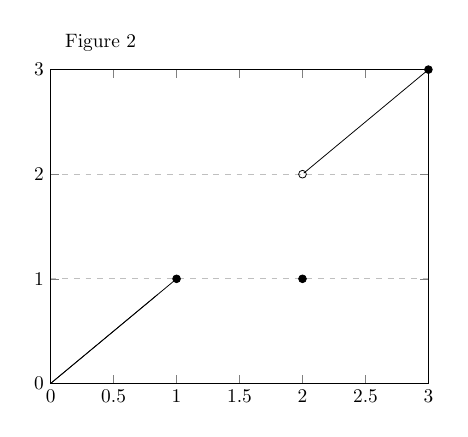
\begin{tikzpicture}[scale=0.7]
\begin{axis}[
title style={text width=18em},
title={Figure 2},
xmin=0,xmax=3,
ymin=0,ymax=3,
legend pos=north west,
ymajorgrids=true,grid style=dashed
]


\addplot[color=black]
coordinates {
(0,0)
(0.5,0.5)
(0.1,0.1)
(0.1,0.1)
(0.2,0.2)
(0.3,0.3)
(0.4,0.4)
(1,1)
};

\addplot[color=black]
coordinates {
(0,0)
(0.5,0.5)
(0.1,0.1)
(0.1,0.1)
(0.2,0.2)
(0.3,0.3)
(0.4,0.4)
(0.85,0.85)
};

\addplot[color=black]
coordinates {
(2.01,2.01)
(3,3)
};


\addplot[color=black,mark=o]
coordinates {
(2,2)
};
\addplot[color=black,mark=*]
coordinates {
(1,1)
};
\addplot[color=black,mark=*]
coordinates {
(2,1)
};
\addplot[color=black,mark=*]
coordinates {
(3,3)
};
\end{axis}

\end{tikzpicture}

\end{center}
\end{itemize}

\bigskip



















\newpage

\subsection{Lebesgue $\Delta \-- $integral and $\Delta \-- $ measure} 


\begin{Def}
\label{rozszerzenie}
Given a function $f: \mathbb{T} \rightarrow \mathbb{R}$, we define the step interpolation $\widehat{f}: [a,b] \rightarrow \mathbb{R} $ as
\begin{center}
$
\widehat{f} (t)  = \left\{ \begin{array}{ll}
f(t), & \textrm{for $t \in \mathbb{T}$}\\
f(t_i), & \textrm{for $ t \in (t_i, \sigma(t_i)), i \in I$}\\
\end{array} \right.
$ .
\end{center}
with $I \subset \mathbb{N}$ and $R= \lbrace t_i \rbrace_{i \in I}$ given in (\ref{11}). 
\end{Def}

The function $\widehat{f}$ extends $f $ to the real interval $[a,b]$ and it allows to establish equivalence between Lebesgue $\Delta \-- $integrable and Lebesgue integrable functions. By using this funtion, we can calculate the Lebesgue $\Delta \-- $integral on arbitrary $\Delta \-- $measurable set as a usual Lebesgue integral on an adequate Lebesgue measurable set. 

\indent
\textbf{\exmp 3.} 
An example of function $p$ defined on time scale $\mathbb{T} = [0,1] \cup \lbrace 2 \rbrace \cup [3,4]$ and \\ $\widehat{p}$ defined on $[0,4]$ is given on Figures 3 and 4. \\

\begin{center}
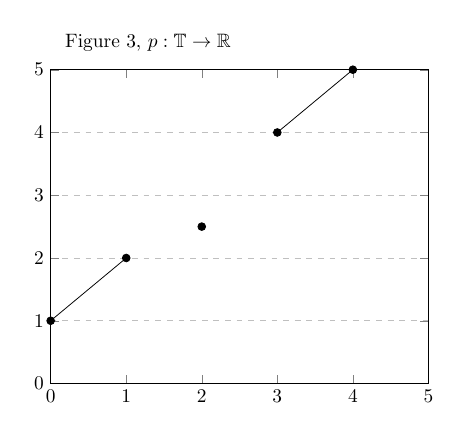
\begin{tikzpicture}[scale=0.7]
\begin{axis}[
title style={text width=18em},
title={Figure 3, $p: \mathbb{T} \rightarrow \mathbb{R}$},
xmin=0,xmax=5,
ymin=0,ymax=5,
legend pos=north west,
ymajorgrids=true,grid style=dashed
]



\addplot[color=black]
coordinates {
(0,1)
(1,2)
};

\addplot[color=black]
coordinates {
(3,4)
(4,5)
};


\addplot[color=black,mark=*]
coordinates {
(0,1)
};
\addplot[color=black,mark=*]
coordinates {
(1,2)
};
\addplot[color=black,mark=*]
coordinates {
(2,2.5)
};
\addplot[color=black,mark=*]
coordinates {
(3,4)
};
\addplot[color=black,mark=*]
coordinates {
(4,5)
};






\end{axis}

\end{tikzpicture}
\end{center}




\begin{center}
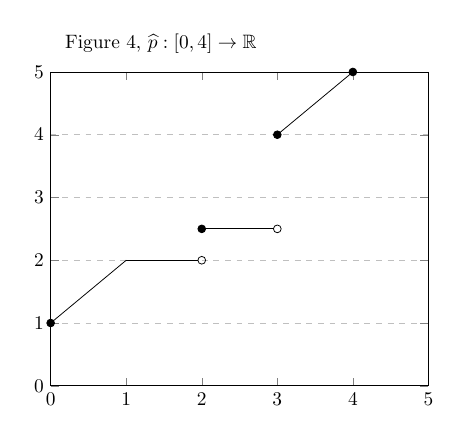
\begin{tikzpicture}[scale=0.7]
\begin{axis}[
title style={text width=18em},
title={Figure 4, $\widehat{p}:[0,4] \rightarrow \mathbb{R}$},
xmin=0,xmax=5,
ymin=0,ymax=5,
legend pos=north west,
ymajorgrids=true,grid style=dashed
]



\addplot[color=black]
coordinates {
(0,1)
(1,2)
};

\addplot[color=black]
coordinates {
(1,2)
(1.95,2)
};

\addplot[color=black]
coordinates {
(3,4)
(4,5)
};

\addplot[color=black]
coordinates {
(2,2.5)
(2.95,2.5)
};



\addplot[color=black,mark=o]
coordinates {
(2,2)
};

\addplot[color=black,mark=*]
coordinates {
(0,1)
};

\addplot[color=black,mark=o]
coordinates {
(3,2.5)
};






\addplot[color=black,mark=*]
coordinates {
(2,2.5)
};
\addplot[color=black,mark=*]
coordinates {
(3,4)
};
\addplot[color=black,mark=*]
coordinates {
(4,5)
};






\end{axis}

\end{tikzpicture}
\end{center}














\indent
\\
\\
\indent
Notice, that continuity of funtion $f:\mathbb{T} \rightarrow \mathbb{R}$ doesn't implies the continuity of function $\widehat{f}:[a,b] \rightarrow \mathbb{R}$. However, we can formulate the following lemma.

\begin{Lemat} Let $f: \mathbb{T} \rightarrow \mathbb{R}$. Then if $f$ is continous on $\mathbb{T}$ and $f(t_i)=f(\sigma(t_i))$ for all $t_i \in R$ with $R$ given in (\ref{11}), then $\widehat{f}$ is continous on $[a,b]$.
\end{Lemat}


\begin{Lemat} \label{Rozszerzenia} Let $f,g : \mathbb{T} \rightarrow \mathbb{R}$. Then 
\begin{itemize}
\item[$(a)$] $\widehat{\vert f \vert^{g}}= \vert \widehat{f} \vert^{\widehat{g}}$ on $ [a,b],$
\item[$(b)$] $\vert \widehat{(f-g)} \vert = \vert (\widehat{f}-\widehat{g})   \vert$  on $ [a,b]$.
\end{itemize}
\begin{proof}
Let $h_1(t)=\vert f(t) \vert^{g(t)}$ and $h_{2}(t)= \vert f(t) - g(t) \vert $. Then  if $t \in \mathbb{T}$, since $\widehat{f}(t)=f(t)$ and $\widehat{g}(t)=g(t)$, we have
\begin{equation}
\nonumber
\widehat{h_1}(t)=h_1(t)= \vert\widehat{f}(t) \vert^{\widehat{g}(t)} \text{ and } \widehat{h_2}(t)=h_2(t)=\vert \widehat{f}(t) - \widehat{g}(t) \vert .
\end{equation}
We now turn to the case when $ t \in (t_i, \sigma(t_i))$ for some $t_i \in R=\lbrace t_i \rbrace_{i \in I}$ given in (\ref{11}) and $I \subset \mathbb{N}$. Then
\begin{equation}
\nonumber
\widehat{h_1}(t)=h_1(t_i)= \vert f(t_i) \vert^{{g}(t_i)} = \vert \widehat{f}(t)) \vert^{\widehat{g}(t)}
\end{equation}
and
\begin{equation}
\nonumber
\widehat{h_2}(t)=h_2(t_i)= \vert f(t_i) - g(t_i) \vert = \vert \widehat{f}(t) - \widehat{g}(t) \vert.
\end{equation} 
\end{proof}
\end{Lemat}

\begin{Twierdzenie} ($[\ref{Rynne}]$, p.1218) We say that $f: \mathbb{T} \rightarrow \mathbb{R}$ is $\Delta \-- $measurable ($\Delta \-- $integrable) if the extension $\widehat{f}: [a,b] \rightarrow \mathbb{R}$ is measurable (integrable) on the interval $[a,b]$ in the usual, Lebesgu'e sense. We let the $L^{1}(\mathbb{T})$ to denote the set of such $\Delta \-- $integrable functions on $\mathbb{T}$. Furthermore, for any $f \in L^{1}(\mathbb{T})$ we define the $\Delta \-- $integral of $f$ by  
\begin{equation}
\label{calkaRozsz}
\int_{\mathbb{T}} f(t) \Delta t = \int_{a}^{b} \widehat{f}(t)dt  
\end{equation}
where integration on the right-hand side is the standard Lebesgu'e integration over the real interval $[a,b] \subset \mathbb{R}$.

\end{Twierdzenie} 






Using above construction, we define a $\Delta \-- $measure and a class of $\Delta \-- $measurable subsets of time-scale $\mathbb{T}$. 



\begin{Def} ($[\ref{Rynne}]$, p.1218)
For any $A \subset \mathbb{T}$, let $\chi_{A}$ denote a characteristic function of $A$. We say that $A$ is $\Delta \-- $measurable if $\chi_{A}$ is measurable (in above sense). If $A$ is $\Delta \-- $measurable, we define the integral of $u \in L^{1}(A)$ over $A$ to be 
\begin{equation}
\nonumber
\int_{A} u(t) \Delta t = \int_{a}^{b} u (t) \chi_{A}(t) \Delta t.
\end{equation}
We also define a $\Delta \-- $measure $\mu_{\Delta}(A)$ of $A$ to be
\begin{equation}
\nonumber
\mu_{\Delta}(A)= \int_{A} 1 \Delta t.
\end{equation}
\end{Def}

\bigskip
\indent



\begin{Lemat} ($[\ref{Rynne}]$, p.1219)
Let $A \subset \mathbb{T}$ be a $\Delta \-- $measurable  set and $\lambda$ be a classical Lebesgue measure. Then, the folllowing properties hold

\begin{equation}
\label{miara_lebesgue+delta}
\mu_{\Delta}(A) = \Sigma_{i \in I_A} \left( \sigma(t_i) - t_i \right) + \lambda(A),
\end{equation}
with
\begin{center}
$I_A= \lbrace i \in I: t_i \in A \cap R \rbrace$,
\end{center}
with $I \subset \mathbb{N}$ and $R = \lbrace t_i \rbrace_{i \in I}$ given in (\ref{11}).
Moreover,
\begin{equation}
\mu_{\Delta}(A) = \lambda(A)
\end{equation}
 if and only if  $A$ does not have any right-scattered points.
\end{Lemat}

\begin{Def} ($[\ref{Agarwal}]$, p.2) Let $A \subset \mathbb{T}$. $A$ is called $\Delta \-- $null set if $\mu_{\Delta}(A)=0.$ We say that some property holds $\Delta \-- $almost everywhere ($\Delta \-- $a.e.) on A or for $\Delta \-- $almost all ($\Delta \-- a.a.$) $t \in A$ if there is $\Delta \-- $null set $E \subset A$ such that this property holds for all $t \in A \setminus E$.
\end{Def}

\begin{Twierdzenie} ($[\ref{Rynne}]$, p.1219)
For each $t_{0}\in \mathbb{T}$, the single point set $\lbrace t_{0} \rbrace$ is $\Delta \-- $measurable and its $\Delta \-- $measure is given by 
\begin{equation}
\nonumber
\mu_{\Delta}(\lbrace t_{0} \rbrace) = \sigma(t_{0})- t_{0}= \mu(t_0). 
\end{equation}
Apart from this,
\begin{equation}
\mu_{\Delta}(\lbrace b \rbrace) = 0
\end{equation}
where $b$ is given in (\ref{kresy}).
\end{Twierdzenie}















Notice that $\Delta \-- $null subsets of $\mathbb{T}$ are only the $\emptyset$ and unions of single $\--$ points set consisted from right-dense points of $\mathbb{T} $. Consequently, we obtain that all subsets of $\Delta \-- $null sets in $\mathbb{T}$ are $\Delta \-- $measurable and that Lebesgue $\Delta \-- $measure $\mu_{\Delta}$ is complete measure. 
\bigskip

The example given below shows that Lebesgue $\Delta \-- $measure is not translation invariant.  \\
\textbf{\exmp  2.} Consider $\mathbb{T}= [0,1] \cup [2,3] \subset \mathbb{R}$ and $A= \lbrace \frac{1}{2} \rbrace \subset \mathbb{T}$. Beacause $t_{0}= \frac{1}{2} \in \mathbb{T}$ is a right-dense point we get
\begin{center}
$\mu_{\Delta}(A)= 0.$
\end{center}
However,
\begin{center}
$\mu_{\Delta}(A+\frac{1}{2})= \mu_{\Delta}(\lbrace 1 \rbrace)= \sigma(1)-1=2-1=1\neq 0.$
\end{center}



\subsection{ $\Delta \-- $derivative}
First, if the time-scale $\mathbb{T}$ has a left-scattered maximum M, then we define 
\begin{equation}
\label{kappa}
\mathbb{T^{\kappa}} = \mathbb{T} \setminus \lbrace M \rbrace.
\end{equation}
Otherwise
\begin{equation}
\nonumber
\mathbb{T}^{\kappa}= \mathbb{T} .
\end{equation}
Generally,
\begin{equation}
\label{T_kappa}
\mathbb{T}^{\kappa}= \left\{ \begin{array}{ll}
\mathbb{T} \setminus (\rho(\sup \mathbb{T}), \sup \mathbb{T}] & \textrm{if $\sup \mathbb{T} < \infty$}\\
\mathbb{T} & \textrm{if $\sup \mathbb{T} = \infty$}
\end{array} \right. .
\end{equation}
Now we consider a function $f: \mathbb{T} \rightarrow \mathbb{R}$ and define the $\Delta \-- $derivative of $f$ at point $t \in \mathbb{T}^{\kappa}$.
\begin{Def} ([\ref{Bohner_1}], p.15) Assume that $f: \mathbb{T} \rightarrow \mathbb{R}$ is a function and let $t\in \mathbb{T}^{\kappa}$. We say that $f$ is $\Delta \-- $differentiable at $t$ if there exists a finite number $f^{\Delta}(t)$  with the property that given any $\epsilon>0$, there is a neighbourhood $U$ of $t$ such that
\begin{equation}
\nonumber
\vert f(\sigma (t)) - f(s) - f^{\Delta}(t) (\sigma(t)-s) \vert \leq \epsilon \vert \sigma(t) -s \vert 
\end{equation}
for all $s \in U$. We call $f^{\Delta}(t)$ the $\Delta \-- $ (or Hilger) derivative of $f$ at $t$.
\end{Def}
Moreover, we say that $f$ is $ \Delta \-- $ (or Hilger) differentiable on $\mathbb{T}^{\kappa}$ provided $f^{\Delta}(t)$ exists for all points $ t \in \mathbb{T}^{\kappa}$. The function $f^{\Delta}: \mathbb{T}^{\kappa} \rightarrow \mathbb{R}$ is then called the $\Delta \-- $derivative of $f$ on $\mathbb{T}^{\kappa}$  

\begin{Twierdzenie}([\ref{Bohner_1}], p.15)
Assume $f: \mathbb{T} \rightarrow \mathbb{R}$ is a function and let $t \in \mathbb{T}^{\kappa}$. Then we the following conditions hold:
\begin{itemize}
\item[(a)] If $f$ is $\Delta \-- $differentiable at t, then f is continous at t.
\item[(b)] If $f$ is continous at t and t is right-scattered, then f is $\Delta \-- $differentiable at t with
\begin{equation}
\nonumber
f^{\Delta}(t)=\frac{f(\sigma (t))-f(t)}{\mu (t)}.
\end{equation}
\item[(c)] If t is a dense point, then f is $\Delta \-- $differentiable if and only if the limit 
\begin{equation}
\nonumber
\lim_{s \rightarrow t } \frac{f(t)-f(s)}{t-s}
\end{equation}
exists as a finite number. In this case
\begin{equation}
f^{\Delta}(t)= \lim_{s \rightarrow t } \frac{f(t)-f(s)}{t-s}.
\end{equation}
\item[(d)] If t is only a right-dense point, then f is $\Delta \-- $differentiable if and only if the limit 
\begin{equation}
\nonumber
\lim_{s \rightarrow t^+ } \frac{f(t)-f(s)}{t-s}
\end{equation}
exists as a finite number. In this case
\begin{equation}
f^{\Delta}(t)= \lim_{s \rightarrow t^+ } \frac{f(t)-f(s)}{t-s}.
\end{equation}
\item[(e)] If f is $\Delta \-- $differentiable at t, then
\begin{equation}
\nonumber
f(\sigma(t))=f(t)+\mu (t) f^{\Delta}(t).
\end{equation}
\end{itemize}

\end{Twierdzenie}
\begin{Def}([\ref{Agarwal}], p.4) A function $f:\mathbb{T} \rightarrow \mathbb{R}$ is said to be absolutely continous on $\mathbb{T}$, if for every $\epsilon>0$, there exists $\delta>0$ such that 
if $\lbrace [a_k, b_k) \cap \mathbb{T} \rbrace_{k=1}^{n} $ with $a_k,b_k \in \mathbb{T}$, $k \in \mathbb{N}$ is a finite pairwise disjoint family of subintervals of $\mathbb{T}$ satifying 
\begin{equation}
\nonumber
\Sigma_{k=1}^n (b_k-a_k)< \delta,
\end{equation}
then
\begin{equation}
\nonumber
\Sigma_{k=1}^n  \vert f(b_k) - f(a_k) \vert < \epsilon.
\end{equation}
\end{Def}
\begin{Def}([\ref{Agarwal}], p.4) \textit{(Fundamental Theorem of Calculus)}  \\ A function $f: \mathbb{T} \rightarrow \mathbb{R}$ is absolutely continous if and only if f is $\Delta \-- $differentiable $\Delta \-- $a.e. on $\mathbb{T}$, $f^{\Delta} \in L^1(\mathbb{T})$ and
\begin{equation}
\nonumber
f(t)=f(a) + \int_{[a,t]_{\mathbb{T}}} f^{\Delta}(t) \Delta t, 
\end{equation}
for $t \in \mathbb{T} $, where $a$ is given in (\ref{kresy}).
\end{Def}
Absolutely continous functions on $\mathbb{T}$ satisfy the integration by parts formula.
\begin{Twierdzenie}  ([\ref{Agarwal}], p.4) If $f,g:\mathbb{T} \rightarrow \mathbb{R}$ are absolutely continous functions, then $f \cdot g$ is absolutely continous on $\mathbb{T}^{\kappa}$ and the following equality is valid
\begin{equation}
\nonumber
\int_{\mathbb{T}}  \left( f^{\Delta}g + f^{\sigma} g^{\Delta} \right) \Delta t = f(b) g(b) - f(a) g(a) = 
\int_{\mathbb{T}}  \left( fg^{\Delta} + f^{\Delta} g^{\sigma} \right) \Delta t,
\end{equation}
where $a,b$ are given in (\ref{kresy}) and $\sigma: \mathbb{T} \rightarrow \mathbb{T}$ is forward-jump operator defined in (\ref{11}).
\end{Twierdzenie}

\section{The space $L^{p(t)}(\mathbb{T})$ }


We consider a bounded time scale $\mathbb{T} \subseteq [a,b]$ and the Lebesgue $\Delta \-- $measure defined on time-scale $\mathbb{T}$.
We denote such measure by $\mu_{\Delta}(\mathbb{T})$. We introduce:
\begin{equation}
\label{E_space}
E = \lbrace u :  \text{u is $\Delta \-- $measurable function on }   \mathbb{T} \rbrace ,
\end{equation}
\begin{equation}
 E_{[a,b]} = \lbrace u : \text{u is measurable function on } [a,b] \rbrace  ,
\end{equation}
\begin{equation}
\label{L_niesk}
 L^{\infty}_{+}(\mathbb{T}) = \lbrace u \in L^{\infty}({\mathbb{T}}):  \essinf_{t \in \mathbb{T}} u(t) \geq 1 \rbrace ,
\end{equation}
\begin{equation}
L^{\infty}_{+}([a,b]) = \lbrace   u \in L^{\infty}([a,b])   \text{ : } \essinf_{t \in [a,b]} u(t) \geq 1 \rbrace . 
\end{equation}
Since now, we always assume that $u \in E$, $p \in L^{\infty}_{+}(\mathbb{T}) \cap E$ and write
\begin{equation}
\label{phi}
\phi(t,s) =  s^{p(t)}    \text{ for all }    t \in \mathbb{T}, s \geq 0,
\end{equation}
\begin{equation}
\label{ro} 
\rho(u) =  \int_{\mathbb{T}} \phi(t, \vert u(t) \vert) \Delta t = \int_{\mathbb{T}} \vert u(t) \vert^{p(t)} \Delta t =\int_{[a,b]}  \vert \widehat{u}(t) \vert^{\widehat{p}(t)} dt ,    
\end{equation}

\begin{equation}
 L^{p(t)}({\mathbb{T}}) = \lbrace u \in E : \lim_{\lambda \rightarrow 0^{+}} \rho(\lambda u) = 0 \rbrace. 
 \end{equation}


\smallskip
\begin{flushleft}
Application of (\ref{calkaRozsz}) enables us to formulate the following lemma
\end{flushleft}
\begin{Lemat} Let $u \in E$ and $p \in L^{\infty}_{+}(\mathbb{T})$. Then:
\begin{itemize}
\item[(a)] $u \in L^{p(t)}(\mathbb{T}) $ if and only if $ \widehat{u} \in L^{\widehat{p}(x)}([a,b]). $
\item[(b)] $p \in L^{\infty}_+ (\mathbb{T}) $ if and only if $ \widehat{p} \in L^{\infty}_+([a,b]). $

\end{itemize}

\begin{proof}
First, we show that condition (a) holds. Let $ u \in L^{p(t)}(\mathbb{T}) $. Then, by Definition \ref{rozszerzenie} and Lemma \ref{rozszerzenie},
\begin{equation}
\nonumber
\widehat{u} \in E_{[a,b]}
\end{equation}
 and
\begin{equation}
\nonumber
0 = \lim_{\lambda \rightarrow 0^{+}} \rho(\lambda u ) = \lim_{\lambda \rightarrow 0^{+}} \int_{\mathbb{T}} \vert \lambda u(t) \vert^{p(t)} \Delta t = \lim_{\lambda \rightarrow 0^{+}} \int_{[a.b]} \vert \lambda \widehat{u}(t) \vert^{\widehat{p}(t)} dt.
\end{equation}
Thus $\widehat{u} \in L^{\widehat{p}(x)}([a,b])$. 
Assume now, that $\widehat{u} \in L^{\widehat{p}(x)}([a,b]) $. Hence, $u \in E$ and 
\begin{equation}
\nonumber
0 \leq \lim_{\lambda \rightarrow 0^{+}} \int_{\mathbb{T}} \vert \lambda u(t) \vert^{p(t)} \Delta t =
\lim_{\lambda \rightarrow 0^{+}} \int_{[a,b]} \vert \lambda \widehat{u}(t) \vert^{\widehat{p}(t)} dt = 0. 
\end{equation} 
\indent
Now, we shall show the part $(b)$. Notice that if $\mathbb{T}$ does not contain any right-scaterred point, then $p=\widehat{p}$ and the thesis is obvious. Assume that $\mathbb{T}$ contains at least one right-scaterred point. Let $p \in L^{\infty}_{+}(\mathbb{T})$. Then 
\begin{equation}
\nonumber
p \in L^{\infty}(\mathbb{T}) \text{ and } \essinf_{t \in \mathbb{T}} p(t) \geq 1.
\end{equation}
Suppose that $\widehat{p} \notin L^{\infty}_{+}([a,b]).$ Then $\widehat{p}$  is unlimited on  $[a,b]$  or 
$\essinf_{t \in [a.b]}\widehat{p}(t)<1.$
However, if one of these cases holds, there must be subset $A \subset [a,b] \setminus \mathbb{T}$ with positive Lebesgue measure in $\mathbb{R}$ such that  $\widehat{p}$ is unlimited on $A$ or $\widehat{p} $ achieves values lower than 1 on $A$. Taking into account Definition \ref{rozszerzenie} we obtain that there exists right-scaterres point $t_0 \in \mathbb{T}$ with such property. As 
\begin{equation}
\nonumber
\mu_{\Delta}(\lbrace t_0 \rbrace) >0,
\end{equation}
we obtain 
\begin{equation}
\nonumber
\essinf_{t \in \mathbb{T}} p(t) <1 .
\end{equation}
It leads to the first implication. \\
\indent
Now, let $\widehat{p} \in L^{\infty}_{+}([a,b]).$ Then
\begin{equation}
\label{p_1}
\widehat{p} \in L^{\infty}([a,b])
\end{equation}
and
\begin{equation}
\label{p_2}
\essinf_{t \in [a,b]} \widehat{p}(t) \geq 1.
\end{equation}
It follows easily that properties (\ref{p_1}) and (\ref{p_2}) are satisfied on $\mathbb{T} \subset [a,b]$. Apart from this, 
\begin{equation}
\nonumber
p(t)=\widehat{p}(t),
\end{equation} 
for $t \in{\mathbb{T}}$. Thus $p\in L^{\infty}_{+}(\mathbb{T})$ and $\essinf_{t \in \mathbb{T}}p(t)\geq 1$. Consequently,
\begin{equation}
\nonumber
p \in L^{\infty}_{+}(\mathbb{T}).
\end{equation}
\end{proof}
\end{Lemat}

\smallskip



\begin{Def} ([\ref{Musielak_modular}], p.1) \label{definicjaModularu}
A functional $\rho : A \rightarrow [0, \infty]$ is called a convex modular, if there hold
\begin{itemize}
\item[($\rho$1)] $\rho(x) = 0$ if and only if $x=0$,
\item[($\rho$2)] $\rho(-x) = \rho(x),$ for $x \in A$,
\item[($\rho$3)] $\rho(\alpha x + \beta y) \leq \alpha \rho(x)+\beta \rho(y)$ for $ x,y \in A,~  \alpha, \beta \geq 0$, $\alpha + \beta = 1$. 
\end{itemize}
\end{Def}
\begin{Def} ([\ref{Musielak_modular}], p.1)
If $\rho$ is a modular over A, then
\begin{equation}
A_{\rho} = \lbrace u \in A: \lim_{\lambda \rightarrow 0^{+}} \rho(\lambda u)=0 \rbrace
\end{equation}
is called a modular space.
\end{Def}






\begin{Twierdzenie} ([\ref{Musielak_modular}], p.108)
\label{klasa_fi}
Let a real function $\varphi$ defined on $\mathbb{T}\times [0, \infty)$ belong to class $\Phi$, e.g. it satisfies the following conditions:
\begin{itemize}
\item[($\Phi$1)] $\varphi (t,\alpha)=0$ if and only if $\alpha=0$,
\item[($\Phi$2)] $\varphi (t,\alpha)$ is a nondecreasing, continous function of $\alpha$, 
\item[($\Phi$3)]$\varphi (t,\alpha)$ is a $\Delta \-- $measurable function of $t$ for all $\alpha \geq 0$. 
\end{itemize}
Then
\begin{equation}
\rho(u) = \int_{\mathbb{T}} \varphi(t,\vert u(t) \vert ) \Delta t
\end{equation}
is a modular in E. If for $\Delta \-- $a.e $t \in \mathbb{T}$ a function $\varphi(t,\alpha)$ is a convex function of $\alpha \geq 0$ , then modular $\rho$ is convex.
\end{Twierdzenie}
It is easy to observe that function 
\begin{equation}
\nonumber
\phi(t, \vert u(t) \vert)= \vert u(t) \vert^{p(t)}
\end{equation}
is a composition of $\Delta \-- $measurable functions. It makes it obvious that it is $\Delta \-- $measurable function of $t$ for every $u \in E_{\rho}$ and that
\begin{equation}
\rho(u) = \int_{\mathbb{T}} \phi (t, \vert u(t) \vert) \Delta t 
\end{equation}
is a modular. Since function $\phi(t,s)$ defined in (\ref{phi}) is a convex function of $s \geq 0$ for $\Delta \-- $a.e $t \in \mathbb{T}$, we obtain convex modulat over $E$.
\begin{Def} ([\ref{Musielak_modular}], p.2) The modular space $A_{\rho}$ is called a generalized Orlicz space and denoted by $L^{\varphi}$, i.e.,
\begin{equation}
L^{\varphi} = \left\lbrace u \in A_{\rho} :
\lim_{\lambda \rightarrow 0^{+}} \int_{\mathbb{T}} \varphi (t,  \vert \lambda u(t) \vert )=0  \right\rbrace.
\end{equation}

\end{Def}


Consequently, we obtain modular space $L^{p(t)}(\mathbb{T})$. Because of description
\begin{equation}
L^{p(t)}(\mathbb{T}) = \left\lbrace u \in E :  \lim_{\lambda \rightarrow 0^{+}}     \int_{\mathbb{T}}\phi(t, \vert \lambda u(t) \vert) \Delta t = 0   \right\rbrace,
\end{equation}
we have that $L^{p(t)}(\mathbb{T})$ is a generalized Musielak-Orlicz space.
By properties of $\phi(t,s)$, we also get
\begin{equation}
\label{another_int}
L^{p(t)}(\mathbb{T}) = \left\lbrace u \in E: \forall \lambda>0, \rho(\lambda u ) < \infty \right\rbrace.
\end{equation}



\bigskip
Observe that for $p \in L^{\infty}_{+}(\mathbb{T})$ we have
\begin{equation}
\label{p_plus_minus}
1 \leq p^{-}=: \essinf_{t \in \mathbb{T}}p(t)= \essinf_{t \in [a,b]}\widehat{p}(t) \leq \esssup_{t \in [a,b]}\widehat{p}(t) = \esssup_{t \in \mathbb{T}}p(t)=: p^{+}< \infty.
\end{equation}

We call $L^{p(t)}(\mathbb{T})$ generalized Lebesgue space on time scale. What's more, we can introduce the norm $\Vert u \Vert_{L^{p(t)}(\mathbb{T})}$ on $L^{p(t)}(\mathbb{T})$ as
\begin{equation}
\Vert u \Vert_{\rho} :=\Vert u \Vert_{L^{p(t)}(\mathbb{T})} = \inf \left\lbrace \lambda > 0 : \rho\left(\frac{u}{\lambda}\right) \leq 1 \right\rbrace. 
\end{equation}
Indeed, if
\begin{equation}
\nonumber
\Vert u \Vert_{\rho} = 0,
\end{equation}
then
\begin{equation}
\nonumber
\rho \left( \frac{u}{\lambda} \right) \leq 1 
\end{equation}
for every $\lambda >0$. Let $\lambda <1$. Then,
\begin{equation}
\nonumber
\frac{1}{\lambda^{p^-}} \int_{\mathbb{T}} \vert u(t) \vert^{p(t)} \Delta t \leq 1
\end{equation}
and
\begin{equation}
\nonumber
\int_{\mathbb{T}} \vert u(t) \vert^{p(t)} \Delta \leq \lambda^{p^-}. 
\end{equation}
Since $\lambda <1$ is arbitrary, we conclude that
\begin{equation}
\nonumber
u(t) = 0,
\end{equation}
for $\Delta \-- $a.e. $t \in \mathbb{T}$.
Now, let $\alpha_0>0$. Then
\begin{equation}
\begin{split}
\Vert \alpha_0 u \Vert_{\rho} = \inf \left\lbrace \lambda \geq 0 : \rho \left( \frac{\alpha_0 u }{\lambda} \right) \leq 1 \right\rbrace = \inf \left\lbrace \lambda \geq 0 : \rho \left( \frac{u}{\frac{\lambda}{\alpha_0}} \right) \leq  1 \right\rbrace \\  =  \alpha_0 \inf \left\lbrace \frac{\lambda}{\alpha_0 } \geq 0 : \rho \left( \frac{u}{\frac{\lambda}{\alpha_0}} \right) \leq 1 \right\rbrace = \alpha_0 \Vert u \Vert_{\rho}.
\end{split}
\end{equation}
Now, for $u,v \in L^{p(t)}(\mathbb{T})$ we denote
\begin{equation}
\nonumber
\alpha_1 = \Vert u \Vert_{\rho} + \alpha_0
\end{equation}
and
\begin{equation}
\nonumber
\alpha_2 = \Vert v \Vert_{\rho} + \alpha_0
\end{equation}
Then, by Definition \ref{definicjaModularu},
\begin{equation}
\begin{split}
\rho \left( \frac{u+v}{\alpha_1 + \alpha_2} \right)= \rho \left( \frac{\alpha_1}{\alpha_1 +\alpha_2} \frac{u}{\alpha_1} + \frac{\alpha_2}{\alpha_1 +\alpha_2} \frac{v}{\alpha_2} \right) \leq 
\frac{\alpha_1}{\alpha_1 + \alpha_2} \rho \left( \frac{u}{\alpha_1} \right) + \frac{\alpha_2}{\alpha_1 + \alpha_2} \rho \left( \frac{v}{\alpha_2} \right)  \\ =   \frac{\alpha_1}{\alpha_1 + \alpha_2} \rho \left( \frac{u}{\Vert u \Vert_{\rho}+\alpha_0} \right) + \frac{\alpha_2}{\alpha_1 + \alpha_2} \rho \left( \frac{v}{ \Vert v \Vert_{\rho}+\alpha_0} \right) \leq \frac{\alpha_1}{\alpha_1 +\alpha_2} + \frac{\alpha_2}{\alpha_1+\alpha_2}=1 .
\end{split}
\end{equation}
Hence,
\begin{equation}
\nonumber
\Vert u + v \Vert_{\rho} \leq \alpha_1+\alpha_2 = \Vert u \Vert + \Vert v \Vert_{\rho}+2\alpha_0.
\end{equation}
Since $\alpha_0$ was arbitrary, we obtain
\begin{equation}
\nonumber
\Vert u + v \Vert_{\rho } \leq \Vert u \Vert_{\rho} + \Vert v \Vert_{\rho}.
\end{equation}


\bigskip
\indent
Notice that, by (\ref{ro}), we obtain
\begin{equation}
\nonumber
\Vert u \Vert_{L^{p(t)}(\mathbb{T})} = \inf \left\lbrace  \lambda>0 : \int_{\mathbb{T}} \left\vert \frac{u(t)}{\lambda} \right\vert^{p(t)} \Delta t \leq 1   \right\rbrace \\ = \inf \left\lbrace  \lambda>0 : \int_{[a,b]} \left\vert \frac{\widehat{u}(t)}{\lambda} \right\vert^{\widehat{p}(t)} dt \leq 1   \right\rbrace.
\end{equation}
Thus,
\begin{equation}
\Vert u \Vert_{L^{p(t)}(\mathbb{T})} = \Vert \widehat{u} \Vert_{L^{\widehat{p}(t)}([a,b])}.
\end{equation}

\begin{Twierdzenie} 
Both $(L^{p(t)}(\mathbb{T})), \Vert \cdot \Vert_{\rho})$  and $ (L^{\widehat{p}(t)}([a,b]), \Vert \cdot \Vert_{L^{\widehat{p}(x)}([a,b])})$ are Banach spaces.
\begin{proof}
By [\ref{oryginal}], we know that $(L^{\widehat{p}(t)}([a,b]), \Vert \cdot \Vert_{L^{\widehat{p}(t)}([a,b])})$ is a Banach space. Now, let $(u_k)_{k \in \mathbb{N}}$ be a Cauchy sequence in $(L^{p(t)}(\mathbb{T})), \Vert \cdot \Vert_{L^{p(t)}(\mathbb{T})})$. Then $\widehat{u_k} \in L^{\widehat{p}(t)}([a.b]) $ for $k \in \mathbb{N}$ and $(\widehat{u}_{k})_{k \in \mathbb{N}}$ is a Cauchy sequence in $L^{\widehat{p}(t)}([a,b]) $. By complecity of $(L^{\widehat{p}(t)}([a,b]), \Vert \cdot \Vert_{L^{\widehat{p}(t)}([a,b])})$, there exists function $\widehat{u} \in L^{\widehat{p}(t)}([a,b])$ such that
\begin{equation}
\nonumber
\lim_{k \rightarrow \infty}\Vert \widehat{u} - \widehat{u_k} \Vert_{L^{\widehat{p}(t)}([a,b])}=0.
\end{equation}
\begin{flushleft}
Denote $u = \widehat{u} |_{\mathbb{T}}$. Then $u \in L^{p(t)}(\mathbb{T})$ and 
\end{flushleft}
\begin{equation}
\nonumber
\lim_{k \rightarrow \infty} \Vert u - u_k \Vert_{\rho} = \lim_{k \rightarrow \infty} \Vert \widehat{u - u_k} \Vert_{L^{\widehat{p}(t)}([a,b])} = \lim_{k \rightarrow \infty} \Vert \widehat{u} - \widehat{u_k} \Vert_{L^{\widehat{p}(t)}([a,b])}=0.
\end{equation}
This completes the proof.
\end{proof}
\end{Twierdzenie} 
\smallskip
Now, observe that for $u \in L^{p(t)}(\mathbb{T})$ and $\lambda>1$ we get
\begin{equation}
\nonumber
 \int_{\mathbb{T}} \vert u(t) \vert^{{p}(t)} \Delta t \leq
\lambda   \int_{\mathbb{T}} \vert u(t) \vert^{p(t)} \Delta t \leq \lambda^{p^-} \int_{\mathbb{T}} \vert u(t) \vert^{p(t)} \Delta t \leq  
\lambda^{p^+} \int_{\mathbb{T}} \vert u(t) \vert^{p(t)} \Delta t
\end{equation}
Thus,
\begin{equation}
\label{3_ciagi_1}
\rho(u) \leq \lambda \rho(u) \leq \lambda^{p^{-}} \rho(u) \leq \rho(\lambda u) \leq \lambda^{p^{+}} \rho(u).
\end{equation}
Similarly, for $\lambda \in (0,1)$ we have
\begin{equation}
\label{3_ciagi_2}
\lambda^{p^{+}} \rho(u) \leq \rho(\lambda u) \leq \lambda^{p^{-}} \rho(u) \leq \lambda \rho(u) \leq \rho(u).
\end{equation}
\indent
Moreover, notice that for every $u \in L^{p(t)}(\mathbb{T})\setminus \lbrace \theta \rbrace $, $\rho(\lambda u)$ is a continous convex even function in $\lambda$ and it increases for $\lambda \in [0, \infty)$.


\begin{Twierdzenie}
\label{rho_1}
 Let $u \in L^{p(t)}(\mathbb{T})\setminus \lbrace \theta \rbrace.$ Then
 \begin{equation}
 \nonumber
 \Vert u \Vert_{\rho} = \alpha>0
 \end{equation}
if and only if 
\begin{equation}
\rho\left(\frac{u}{\alpha}\right)=1.
\end{equation}
\end{Twierdzenie}
\begin{proof} 
Let $u \in L^{p(t)}(\mathbb{T})\setminus \left\lbrace \theta \right\rbrace $. First, assume that $\Vert u \Vert_{\rho} =\alpha$. Then
\begin{equation}
\nonumber
\alpha = \inf \lbrace \lambda > 0 : \rho \left( \frac{u}{\lambda} \right) \leq 1 \rbrace .
\end{equation}
If we denote,
\begin{equation}
\nonumber
 \rho_u(\lambda) =\rho \left( \frac{u}{\lambda} \right) = \int_{\mathbb{T}} \left\vert \frac{u(t)}{\lambda} \right\vert^{p(t)}  \Delta t, 
\end{equation}
then $\rho_u$ is continous and decreases on $(0, \infty)$. Observe that 
\begin{equation}
\nonumber 
\alpha = \inf \lbrace \lambda : \lambda \in \rho^{-1}_u \left( [0, 1 ] \right) \rbrace.
\end{equation}
Continuity and monotocity of $\rho_u$ leads to
\begin{equation}
\nonumber
1=\rho_u(\alpha) = \rho\left(\frac{u}{\alpha}\right).
\end{equation}

Now, assume that $\rho(\frac{u}{\alpha})=1$  for some $\alpha>0$. Observe, that then there exists $\beta \in \mathbb{R}$ such that
\begin{equation}
\nonumber
\Vert u \Vert_{\rho} = \beta \leq \alpha  
\end{equation}
and
\begin{equation}
\nonumber
\rho_{u}(\beta) = \rho \left( \frac{u}{\beta} \right) \leq 1 = \rho \left( \frac{u}{\alpha} \right) = \rho_{u}(\alpha). 
\end{equation}
By monotocity of $\rho_{u}$, we obtain that 
\begin{equation}
\nonumber
 \beta \geq \alpha.
\end{equation}

Finally,
\begin{equation}
\nonumber
\Vert u \Vert_{\rho} = \beta = \alpha. 
\end{equation}
\end{proof}

\begin{Twierdzenie}
\label{szacowania_u}
Let $u \in L^{p(t)}(\mathbb{T}) \setminus \lbrace \theta \rbrace.   $ Then 
\begin{enumerate}
\item[(a)] $\Vert u \Vert_{\rho} < 1 (=1,~ >1) \Leftrightarrow \rho(u) <1 (=1,~ >1)$.
\item[(b)] If $\Vert u \Vert_{\rho} > 1 $, then $\Vert u \Vert_{\rho}^{p^{-}} \leq \rho(u) \leq \Vert u \Vert_{\rho}^{p^{+}}$,
\item[(c)] If $\Vert u \Vert_{\rho} < 1 $, then $\Vert u \Vert_{\rho}^{p^{+}} \leq \rho(u) \leq \Vert u \Vert_{\rho}^{p^{-}}$.
\end{enumerate}

\end{Twierdzenie}

\begin{proof}
First, we show (a). Assume that
\begin{equation}
\nonumber
\Vert u \Vert_{\rho} = \alpha <1 .
\end{equation} 
Theorem \ref{rho_1} and monotocity of the modular enables us to write
\begin{equation}
\nonumber
\rho(u) < \rho\left(\frac{u}{\alpha}\right)=1.
\end{equation}
Similar considerations can be applied when $\Vert u \Vert_{\rho}>1$ or $\Vert u \Vert_{\rho}=1$. \\
\indent
Now, we focus our attenion on (b). Assume that
\begin{equation}
\nonumber
\Vert u \Vert_{\rho}= \alpha >1.
\end{equation}
Applying Theorem \ref{rho_1} again, we conclude
\begin{equation}
\nonumber
1 = \rho \left( \frac{u}{\alpha } \right)  = \int_{\mathbb{T}} \left(  \frac{\vert u(t) \vert}{\alpha } \right)^{p(t)} \Delta t \leq \frac{1}{\alpha^{p^-}} \int_{\mathbb{T}} \vert u(t) \vert^{p(t)} \Delta t = \frac{1}{\alpha^{p^-}}  \rho(u).
\end{equation}
Moreover, we get
\begin{equation}
\nonumber
1 = \rho \left( \frac{u}{\alpha } \right) \geq \frac{1}{\alpha^{p^+}}  \int_{\mathbb{T}} \vert u(t) \vert^{p(t)} \Delta t = \frac{1}{a^{p^+}}  \rho(u).
\end{equation}
In general, we have
\begin{equation}
\nonumber
\Vert u \Vert^{p^-} = \alpha^{p^-} \leq \rho(u) \leq \alpha^{p^+} = \Vert u \Vert^{p^+}.
\end{equation}
The proof for (c) may be handled in much the same way as (b).
\end{proof}

\smallskip

To obtain our next result, we will need the theorem and lemma below.

\begin{Twierdzenie}
\label{rownowaznosc_1}
Let $\rho$ be a modular on $E $. If $u, ~u_k \in E$ for $k \in \mathbb{N}$, then the condition 
\begin{equation}
\nonumber
\Vert u_k - u \Vert_{\rho} \rightarrow 0
\end{equation}
 as $k \rightarrow \infty$ is equivalent to the condition  
\begin{equation}
\nonumber
\rho (\lambda (u_k - u)) \rightarrow 0
\end{equation} 
as $k \rightarrow \infty $ for every $\lambda \geq 0$.
\begin{proof}
First, assume that
\begin{equation}
\nonumber
\lim_{k \rightarrow \infty} \Vert u - u_k \Vert_{\rho} = 0.
\end{equation}
Then
\begin{equation}
\nonumber
\lim_{k \rightarrow \infty} \Vert \lambda ( u - u_k) \Vert_{\rho} = 0 
\end{equation}
for all $\lambda \geq 0$. Now, let $\lambda \geq 0$ and $\epsilon \in (0,1)$. Then, there exists $k_0 \in \mathbb{N}$ such that for $k>k_0$
\begin{equation}
\nonumber
\Vert \lambda \left(u_k -u \right) \Vert_{\rho} < \epsilon,
\end{equation}
By Thorem \ref{szacowania_u}, for  every $k>k_0$ we get
\begin{equation}
\nonumber
\rho \left( \lambda  \left( u_k - u  \right) \right) \leq \Vert \lambda (u_k - u ) \Vert_{\rho}^{p^-} \leq \Vert \lambda (u_k - u ) \Vert_{\rho}  < \epsilon.
\end{equation}
Thus 
\begin{equation}
\nonumber
\lim_{k \rightarrow \infty } \rho \left( \lambda  \left( u_k - u  \right) \right) = 0.
\end{equation}
Beacause $\lambda \geq 0$ and $\epsilon \in (0,1)$ were arbitrary, we obtain the first implication. \\
\indent
Assume now that
\begin{equation}
\nonumber
\lim_{k \rightarrow \infty} \rho(\lambda \left( u_k - u \right) ) = 0 
\end{equation}
for every $\lambda \geq 0$. Then there exists $k_0 \in \mathbb{N}$ such that for $k>k_0$
\begin{equation}
\nonumber 
 \rho \left( \frac{  \left( u_k - u  \right)}{\frac{1}{\lambda}} \right)  =\rho(\lambda \left( u - u_k \right) ) < 1,
\end{equation}
for arbitrary $\lambda > 0$. Thus,
\begin{equation}
\nonumber
\Vert u - u_k \Vert_{\rho} \leq \frac{1}{\lambda}
\end{equation}
for $k>k_0$ and every $\lambda >0$.
This gives
\begin{equation}
\nonumber
\lim_{k \rightarrow \infty} \Vert u_k - u \Vert_{\rho} = 0.
\end{equation}
\end{proof}



\end{Twierdzenie}



By (\ref{3_ciagi_1}) and (\ref{3_ciagi_2}), we obtain the results below.
\begin{Lemat}
\label{3_ciagi}
Let $u, u_k \in E$ for $k \in \mathbb{N}$. If 
\begin{equation}
\nonumber
\lim_{k \rightarrow \infty} \rho(u_k - u)=0,
\end{equation} then 
\begin{equation}
\nonumber
\lim_{k \rightarrow \infty} \rho( \lambda  ( u_k - u))=0 
\end{equation}
for all $\lambda >0$.
\end{Lemat}










\begin{Twierdzenie}
\label{warunki}
Let $u, u_k \in L^{p(t)}(\mathbb{T}),~ k =1,2,...$ . Then the following statements are equivalent to each other:
\begin{enumerate}
\item[(a)] $ \lim_{k \rightarrow \infty} \Vert u_k - u \Vert_{\rho}=0,$
\item[(b)] $ \lim_{k \rightarrow \infty} \rho(u_k - u)=0 $.
\end{enumerate}
\begin{proof}
First, assume that condition $(a)$ holds. We conclude from Theorem \ref{rownowaznosc_1} that
\begin{equation}
\nonumber
\lim_{k \rightarrow \infty} \rho(\lambda (u_k - u))=0 \text{ for all } \lambda>0.
\end{equation}
Especially, it is satisfied for $\lambda =1$ and thus condition $(b)$ is fullfield. 
Now, if condition $(b)$ holds then Lemma \ref{3_ciagi} forces that 
\begin{equation}
\nonumber
\lim_{k \rightarrow \infty} \rho( \lambda  ( u_k - u))=0,
\end{equation}
 for all $\lambda >0$. Taking into account the equivalence in Thoerem \ref{rownowaznosc_1}, we obtain (a).
\end{proof}
\end{Twierdzenie}

\begin{Twierdzenie} 
\label{podciag_pw_zbiezny}
Let $u, u_k \in L^{p(t)}(\mathbb{T}),~ k \in \mathbb{N}$. 
If 
\begin{equation}
\lim_{k \rightarrow \infty} \Vert u_k - u \Vert_{\rho}=0,
\end{equation}
then 
\begin{equation}
u_k \rightarrow u 
\end{equation}
in $\Delta \-- $measure and it contains  subsequence $u_{k_i}$ that is  $\Delta \-- $a.e. convergent on $\mathbb{T}$.
\end{Twierdzenie}
\begin{proof}
Let $\alpha>0$. First, define the measure
\begin{equation}
\label{new_measure}
\vartheta (A) = \int_{A} \phi (t, \alpha) \Delta t,
\end{equation}
where $A \subset \mathbb{T}$ and  the function $\phi$ is defined in (\ref{phi}).
Next, we notice that $\Delta \-- $measure is absolutly continous with respect to the measure given in (\ref{new_measure}). If for $A \subset \mathbb{T}$ holds
\begin{equation}
\nonumber
\vartheta(A)=0,
\end{equation}
 by (\ref{miara_lebesgue+delta}), we are able to conclude that the set $A$ cannot contain any right-scaterred points and
\begin{equation}
\nonumber
\int_{A} \phi(t,\alpha)\ dt =0,
\end{equation} 
for every $\alpha>0$. As $\phi$ is non-negative function, we obtain that 
\begin{equation}
\nonumber
\lambda(A)= \mu_{\Delta}(A) = 0 .
\end{equation}	
Now, if 
\begin{equation}
\nonumber
\lim_{k \rightarrow \infty} \Vert u_k - u \Vert_{\rho}=0,
\end{equation}
then by Theorem \ref{warunki}, for every $\epsilon>0$ there exists $k_0 \in \mathbb{N}$ such that for $k > k_0$ we have
\begin{equation} 
\nonumber
 \rho(u_k-u)< \epsilon^{2p^+}.
\end{equation}
Now, let $\epsilon \in (0,1)$. We denote
\begin{equation}
\nonumber
 A_{k}= \lbrace t \in \mathbb{T} : \vert u_k (t) - u(t) \vert \geq \epsilon \rbrace,
\end{equation} 
 for $k >k_0$. Then, 
\begin{equation}
\nonumber
 \int_{A_k} \phi (t, \epsilon) \Delta t = \int_{A_k} \epsilon^{p(t)} \Delta t \leq \int_{A_k}  \vert u_k (t) - u(t) \vert^{p(t)} \Delta t \leq   \rho(u_k-u) <   \epsilon^{2p^+}
\end{equation} 
for $k>k_0.$ Thus,
\begin{equation}
\nonumber
 \epsilon^{p^+} \mu_{\Delta} (A_k)  =  \int_{A_k} \epsilon^{p^+} \Delta t  \leq \int_{A_k} \epsilon^{p(t)} \Delta t    \leq \epsilon^{2p^+}
\end{equation}
and 
\begin{equation}
\nonumber
\mu_{\Delta} (A_k)\leq \epsilon^{p^+},
\end{equation}
for $k>k_0$.
Consequently, we obtain
\begin{equation}
\nonumber
 \lim_{k \rightarrow \infty} \mu_{\Delta}(A_k) = 0.
\end{equation} 
Hence, the sequence $(u_k)_{k \in \mathbb{N}}$ is convergent to $u$ in $\Delta \-- $measure on $\mathbb{T}$. Moreover, because $(u_k)_{k \in \mathbb{N}}$ is a Cauchy sequence in $(L^{p(t)}(\mathbb{T}), \Vert \cdot \Vert_{\rho})$, we can similarly show that $(u_k)_{k \in \mathbb{N}}$ is Cauchy sequence in $\Delta \-- $measure. By Riesz theorem about subsequence, $(u_k)_{k \in \mathbb{N}}$ contains  subsequence $u_{k_i}$ that is convergent  $\Delta \-- $a.e. on $\mathbb{T}$. 
\end{proof}








We now discuss the uniform convexivity of $L^{p(t)}(\mathbb{T})$. First, let's consider the following lemma:
\begin{Lemat} ([\ref{Brezis}], p.103)
\label{jednostajna_wypuklosc}
Let $p \in L^{ \infty}_{+}(\mathbb{T})$ and 
\begin{equation}
p(t) \geq 2,
\end{equation}
for $\Delta \-- $a.e. $t \in \mathbb{T}$. Then,
\begin{equation}
\left\vert \frac{\alpha+ \beta}{2} \right\vert^{p(t)} + \left\vert \frac{\alpha - \beta}{2} \right\vert^{p(t)} \leq \frac{1}{2} \left( \vert \alpha \vert^{p(t)} + \vert \beta \vert^{p(t)} \right),
\end{equation}
for every $\alpha, \beta \in \mathbb{R}$ and $\Delta \-- $a.e. $t \in \mathbb{T}$.
\end{Lemat}

\begin{Def}([\ref{Brezis}], p.76) A Banach space ($X$, $\Vert \cdot \Vert$) is said to be uniformly convex if for every $\epsilon >0$ there exists $\delta >0$ such that  for every $x,y \in X$ with $\Vert x \Vert \leq 1 $, $\Vert y \Vert \leq 1$ and $\Vert x-y \Vert > \epsilon $, we have
\begin{equation}
\nonumber
\left\Vert \frac{x+y}{2} \right\Vert < 1 - \delta . 
\end{equation}
\end{Def}

\begin{Twierdzenie} 
\label{refleksywnoc}
([\ref{Brezis}], p.77) Every uniformly convex Banach space is reflexive. 
\end{Twierdzenie}


By Lemma \ref{jednostajna_wypuklosc} and Theorem \ref{refleksywnoc}, we obtain:
\begin{Twierdzenie} 
\label{refleksywnosc_p>1}
Let $p \in L^{ \infty}_{+}(\mathbb{T})$ and 
\begin{equation}
\nonumber
p(t) \geq 2,
\end{equation}
for $\Delta \-- $a.e. $t \in \mathbb{T}$, then $L^{p(t)}(\mathbb{T})$ is uniformly convex and thus relfexive. 

\begin{proof}
Let $\epsilon >0$ and $u,v \in L^{p(t)}(\mathbb{T})$ such that $\Vert u \Vert_{\rho} \leq 1$, $\Vert v \Vert_{\rho} \leq 1$ and $\Vert u -v \Vert_{\rho}> \epsilon$. Then, by Theorem \ref{szacowania_u}, we get that $\rho(u)\leq 1 $, $\rho(v) \leq 1$. Using, Lemma \ref{jednostajna_wypuklosc}, we obtain that
\begin{equation}
\nonumber
\left\vert \frac{u(t)+v(t)}{2} \right\vert^{p(t)} + \left\vert \frac{u(t)-v(t)}{2} \right\vert^{p(t)} \leq \frac{1}{2} \left( \vert u(t) \vert^{p(t)} + \vert v(t) \vert^{p(t)} \right)
\end{equation}
for $\Delta \-- $a.e. $t \in \mathbb{T}$. Integrating it both sides and applying Theorem \ref{szacowania_u}, we have
\begin{equation}
\nonumber
\rho\left(\frac{u+v}{2}\right) + \rho\left(\frac{u-v}{2}\right) \leq \frac{1}{2} \left( \rho(u) + \rho(v) \right) \leq 1.
\end{equation}
Hence,
\begin{equation}
\rho \left(\frac{u+v}{2} \right) \leq 1 - \rho \left(\frac{u-v}{2} \right).
\end{equation}
Now, assume that $\epsilon \in (0,1)$. Then
\begin{equation}
\nonumber
\frac{1}{\epsilon^{p^+}} \rho(u-v) = \frac{1}{\epsilon^{p^+}} \int_{\mathbb{T}} \vert u(t) - v(t) \vert^{p(t)} \Delta t \geq \rho \left( \frac{u-v}{\epsilon} \right) \geq 1.
\end{equation}
Thus,
\begin{equation}
\label{47}
\rho(u-v) \geq \epsilon^{p^+}.
\end{equation}
By
\begin{equation}
\nonumber
\rho \left( \frac{u-v}{2} \right) = \int_{\mathbb{T}} \left\vert \frac{u(t)-v(t)}{2} \right\vert^{p(t)} \Delta t \geq \frac{1}{2^{p^+}} \rho(u-v) 
\end{equation}
and $(\ref{47})$, we obtain
\begin{equation}
\nonumber
\rho\left( \frac{u+v}{2} \right) \leq 1 - \rho \left( \frac{u-v}{2} \right) \leq 1 - \frac{\epsilon^{p^+}}{2^{p^+}} < 1.
\end{equation}
As a result, for $\delta=\frac{\epsilon^{p^+}}{2^{p^+}}$, by Theorem \ref{szacowania_u}, there holds
\begin{equation}
\label{48}
\left\Vert \frac{u+v}{2} \right\Vert_{\rho} < 1 - \delta.
\end{equation}
If we apply similar considerations for $\epsilon>1$, we obtain inequality ($\ref{48}$) with $\delta=\frac{\epsilon^{p^-}}{2^{p^+}} $.


\end{proof}
\end{Twierdzenie}




\indent
 Now, it is our purpose to receive reflexivity of spaces $L^{p(t)}(\mathbb{T})$ with another conditions about function $p$. For this, reason we consider the theory of conjugate functions and complementary in the sense of Young. Firstly, we establish the following Lemmas.

\begin{Lemat}
\label{lemat_holder_1}
$([\ref{Musielak_modular}], p.48)$ Let $p,q:\mathbb{T} \rightarrow \mathbb{R}$ be a conjugative functions on $\mathbb{T}$, e.g.  
\begin{equation}
\label{pq_sprz}
\frac{1}{p(t)} + \frac{1}{q(t)} =1 ,
\end{equation}
for $\Delta \-- $a.e $t \in \mathbb{T}$.
Then 
\begin{equation}
\label{holder_11}
\alpha \beta \leq \frac{\alpha^{p(t)}}{p(t)} + \frac{\beta^{q(t)}}{q(t)} \leq \frac{\alpha^{p(t)}}{p^-} +   \frac{\beta^{q(t)}}{q^-},
\end{equation}
for $\alpha, \beta >0$ and $\Delta \-- $a.e. $t \in \mathbb{T}$.
\end{Lemat}
\begin{Lemat}
\label{lemat_holder_2}
 Let $p,q:\mathbb{T} \rightarrow \mathbb{R}$ be a conjugative functions on $\mathbb{T}$, e.g.  
satisfying equality defined in (\ref{pq_sprz}).
Then 
\begin{equation}
\label{holder_21}
\nonumber
\int_{\mathbb{T}} \vert u(t) v(t) \vert \Delta t \leq \frac{1}{p^-} \int_{\mathbb{T}} \vert u(t) \vert^{p(t)} \Delta t + \frac{1}{q^-} \int_{\mathbb{T}} \vert v(t) \vert^{q(t)} \Delta t ,
\end{equation}
for $u,v \in E$, where $E$ is defined in (\ref{E_space}).
\begin{proof}
Inequality (\ref{holder_11}) enables us to write
\begin{equation}
\label{bothSides}
\vert u(t) v(t) \vert \leq \frac{\vert u(t) \vert^{p(t)}}{p^-} + \frac{\vert v(t)\vert^{q(t)}}{q^-},
\end{equation}
for $\Delta \-- $a.e. $t \in \mathbb{T}$.
Integrating (\ref{bothSides}) both sides, we obtain
\begin{equation}
\label{poprawiona_nierownosc}
\int_{\mathbb{T}} \vert u(t) v(t) \vert \Delta t \leq \frac{1}{p^-} \int_{\mathbb{T}} \vert u(t) \vert^{p(t)} \Delta t + \frac{1}{q^-} \int_{\mathbb{T}} \vert v(t) \vert^{q(t)} \Delta t .
\end{equation}
\end{proof}
\end{Lemat}


\begin{Twierdzenie}
\label{zanurzanie_;[}
 Let $p_1, p_2 \in L^{\infty}_{+}(\mathbb{T})$ be such that conditions defined in (\ref{p_plus_minus}) are satisfied for functions $p_1,p_2$ and $p_1(t) \leq p_2(t)$ $\Delta \--$a.e on $\mathbb{T}$. Then $L^{p_2(t)}(\mathbb{T}) \subset L^{p_1(t)}(\mathbb{T})$.
\end{Twierdzenie}
\begin{proof}
Let $u \in L^{p_2(t)}(\mathbb{T})$. Assume that for $\Delta \-- $a.e. $t \in \mathbb{T}$, we have
\begin{equation}
p_1(t) \leq p_2(t).
\end{equation}
Then,
\begin{equation}
\label{p1_skonczone}
 \int_{\mathbb{T}} \vert  u(s) \vert^{p_2(s)} \Delta s < \infty. 
\end{equation}
\indent
Now, if we consider inequality (\ref{poprawiona_nierownosc}) with
\begin{equation}
\nonumber
u= \vert u(t) \vert^{p_1(t)},~ v \equiv 1,~p(t) = \frac{p_2(t)}{p_1(t)},
\end{equation}
 for $ \Delta \--$a.e. $ t \in \mathbb{T}$, we obtain
\begin{equation}
\nonumber
\int_{\mathbb{T}} \vert u(t) \vert^{p_1(t)} \Delta t \leq  \frac{1}{p^-} \int_{\mathbb{T}} \vert u(t) \vert^{p_2(t)} \Delta t + \frac{1}{q^-} \mu_{\Delta}(\mathbb{T}) < \infty.
\end{equation}
By (\ref{p1_skonczone}), we have
\begin{equation}
\nonumber
 \int_{\mathbb{T}} \vert  u(s) \vert^{p_1(s)} \Delta s < \infty. 
\end{equation}
As a result, $u \in L^{p_1(t)} \left( \mathbb{T}\right)$.
\end{proof}
\bigskip
Now, we shall discuss the conjugative space $ \left( L^{p(t)} \left( \mathbb{T}\right) \right)^{*}$.
\begin{Lemat} $([\ref{Musielak_modular}], p.82)$ If a function $ \varphi$ belongs to class $\Phi$ defined in Theorem \ref{klasa_fi} and it is a convex function of the variable $\alpha$ for every $t \in \mathbb{T}$, then $\varphi$ is of the form
\begin{equation}
\label{young_1}
\varphi(t,\alpha) = \int_{0}^{\vert \alpha \vert} g(t, s) \Delta s,
\end{equation} 
where $g(t,u)$ is right-handed derivative of $\varphi(t,u)$ for a fixed $t \in \mathbb{T}$.
\end{Lemat}
\begin{Def} $([\ref{Musielak_modular}], p.82)$ We say that a function $\varphi \in \Phi$ is N-function (or $\varphi \in N$), if $\varphi$ is a convex function of $\alpha$ for every $t \in \mathbb{T}$ and 
\begin{itemize}
\item[(N1)] $\lim_{\alpha \rightarrow 0^+} \frac{\varphi(t,\alpha)}{\alpha}=0,$
\item[(N2)] $\lim_{\alpha \rightarrow \infty}\frac{\varphi(t,\alpha)}{\alpha}=\infty. $
\end{itemize} 
\end{Def}
\begin{Def}$([\ref{Musielak_modular}], p.82)$ Let $\varphi \in N$ be of the form defined in (\ref{young_1}) and 
\begin{equation}
g^{*}(t,\alpha)=\sup \lbrace s : g(t, s) \leq \alpha \rbrace .
\end{equation}
 Then the function
\begin{equation}
\varphi^*(t,\alpha) = \int_{0}^{\vert \alpha \vert} g^*(t,s)\Delta s
\end{equation}
is called a complementary of $\varphi$ in the sense of Young.
\end{Def}

\begin{Twierdzenie}([\ref{Musielak_analysis}], p.104) Let  $\varphi^*$ be complementary function in the sense of Young to $\varphi$. Then, $\varphi^*$ and $\varphi$ are convex and they satisfy Young inequality
\begin{equation}
\label{young_inequality}
\alpha \beta \leq \varphi (\alpha) +\varphi^* (\beta),
\end{equation}
for all $\alpha, $ $\beta>0$.
\end{Twierdzenie}
\bigskip
\indent
Set
\begin{equation}
\phi_{p}(t,s)= \frac{1}{p(t)} s^{p(t)}, ~t \in \mathbb{T}, s>0.
\end{equation}
Then $\phi_p \in \Phi$. Moreover,
\begin{equation}
\nonumber
\lim_{s \rightarrow 0^+} \frac{\phi_p (t,s)}{s}= \lim_{s \rightarrow 0^+} \frac{s^{p(t)}}{p(t) s}= \lim_{s \rightarrow 0^+} \frac{1}{p(t)} s^{p(t)-1}=0
\end{equation} 
and
\begin{equation}
\nonumber
\lim_{s \rightarrow \infty} \frac{\phi_p (t,s)}{s} = \lim_{s \rightarrow \infty} \frac{1}{p(t)} s^{p(t)-1} = \infty.
\end{equation}
Consequently, $\phi_p \in N$. 
Writing 
\begin{equation}
\rho_{p}(u) = \int_{\mathbb{T}} \phi_p (t, \vert u(t) \vert ) \Delta t
\end{equation}
and 
\begin{equation}
\label{nowa_norma}
\Vert u \Vert_{p} =  \inf  \lbrace \lambda > 0 : \rho_{p} \left( \frac{u}{\lambda}  \right) \leq 1 \rbrace,
\end{equation}
we obtain an equivalent norm to $\Vert \cdot \Vert_{\rho}$ on $L^{p(t)}(\mathbb{T})$. \\
\indent
Now, notice that
\begin{equation}
\nonumber
\phi_{p}(t,s) = \frac{1}{p(t)} s^{p(t)} = \int_{0}^{\vert s \vert} r^{p(t)-1} \Delta r
\end{equation}
and
\begin{equation}
\nonumber
\sup \lbrace s : s^{p(t)-1} \leq r \rbrace = \sup \lbrace s : s \leq r^{\frac{1}{p(t)-1}} \rbrace= r^{\frac{1}{p(t)-1}}.
\end{equation}
Thus
\begin{equation}
\phi_p^* (t,s) =\int_{0}^{\vert s \vert} r^{\frac{1}{p(t)-1}} \Delta r = \frac{p(t)-1}{p(t)} s^{\frac{p(t)}{p(t)-1}} = \frac{1}{q(t)} s^{q(t)},
\end{equation}
where $q: \mathbb{T} \rightarrow \mathbb{R} $ is the conjugative function to $p$ on $\mathbb{T}$.
Writing 
\begin{equation}
\nonumber
\rho_{p}^*(v) = \int_{\mathbb{T}} \frac{1}{q(t)} \vert v(t) \vert^{q(t)} \Delta t = \int_{\mathbb{T}} \phi_p^* (t, \vert v(t) \vert ) \Delta t,
\end{equation}
we obtain
\begin{equation}
\nonumber
L^{q(t)}(\mathbb{T}) = \lbrace v \in E : \lim_{\lambda \rightarrow 0^+} \rho_q^* (v) = 0 \rbrace = \lbrace v \in E : \int_{\mathbb{T}} \vert v(t) \vert^{q(t)} \Delta t < \infty \rbrace. 
\end{equation}
Observe that $\phi_p$ and $\phi_p^*$ are locally integrable. Consequently, using Corolarry 13.14 and Theorem 13.17 in [\ref{Musielak_modular}] we can formulate the following theorems.
\begin{Twierdzenie}
\label{Twierdzenie18}
\label{funkcjonal_Tw}
 For every $v \in L^{q(t)}(\mathbb{T})$, f defined by
\begin{equation}
\label{funkcjonal}
f(u) = \int_{\mathbb{T}} u(t) v(t) \Delta t , \text{ u } \in L^{p(t)}(\mathbb{T})
\end{equation}
is u continous linear functional over $L^{p(t)}(\mathbb{T})$.
\end{Twierdzenie} 
\begin{Twierdzenie} For every continous functional f on $L^{p(t)}(\mathbb{T})$, there is a uniqe element $v \in L^{q(t)}(\mathbb{T})$ such that f is exactly defined by (\ref{funkcjonal}).
\end{Twierdzenie}
Consequently, the following theorem holds.

\begin{Twierdzenie}
 $(L^{p(t)}(\mathbb{T}))^* = L^{q(t)}(\mathbb{T})$.
\end{Twierdzenie}
\bigskip

Apart from this, for Banach spaces we can formulate lemma.
\begin{Lemat}
\label{reflexive_dual}
([\ref{Brezis}], p.)A Banach $X$ space is relfexive if and only if its dual space $X^{*}$ is relfexive.
\end{Lemat}
\indent
By Theorem \ref{refleksywnosc_p>1}, we know that if $p \in L^{\infty}_{+}(\mathbb{T})$ and
\begin{equation}
\nonumber
p(t) \geq 2,
\end{equation}
for $\Delta \-- $a.e. $t \in \mathbb{T}$, then $L^{p(t)}(\mathbb{T})$ is reflexive. Notice, that
\begin{equation}
(L^{p(t)}(\mathbb{T}))^{*}= L^{q(t)}(\mathbb{T}),
\end{equation}
where
\begin{equation}
\nonumber
q(t) \in (1,2],
\end{equation}
for $\Delta \-- $a.e. $t \in \mathbb{T}$. Applying Lemma \ref{reflexive_dual},
we obtain that $L^{p(t)}(\mathbb{T})$ is reflexive for function $p \in L^{\infty}_{+}(\mathbb{T})$ satisfying condition
\begin{equation}
\nonumber
p(t) \in (1,2],
\end{equation}
for $\Delta-$a.e. $t \in \mathbb{T}$.

\indent
We know that for a Banach space $(X, \Vert \cdot \Vert)$ we can construct the norm $\Vert \cdot \Vert^{'}$ on its conjugate space $X^*$ given by
\begin{equation}
\Vert x^* \Vert^{'} = \sup \lbrace x^* (x) : x \in X \text{ and } \Vert x \Vert \leq 1 \rbrace.
\end{equation} 
Let us consider the space $X = L^{p(t)}(\mathbb{T})$ equipped with the norm $\Vert \cdot \Vert_{\rho_p}$. If
\begin{equation}
\nonumber
v \in X^*= L^{q(t)}(\mathbb{T}),~ u \in X,
\end{equation}
we have
\begin{equation}
\nonumber
v(u) = \int_{\mathbb{T}} u(t) v(t) \Delta t .
\end{equation}
\indent
Young inequality $(\ref{young_inequality})$ enables us to formulate theorem below for $\Vert \cdot \Vert_{q}$ and $\Vert \cdot \Vert^{'}$ defined on $L^{q(t)}(\mathbb{T})$.
\begin{Twierdzenie} Let $v \in L^{q(t)}(\mathbb{T})$. Then
\begin{equation}
\nonumber
\Vert v \Vert_{q} \leq \Vert v \Vert^{'} \leq \left( \frac{1}{p^-}+ \frac{1}{q^-} \right) \Vert v \Vert_{q}.
\end{equation}
\begin{proof}
For $v \in L^{q(t)}(\mathbb{T}) $, $u \in L^{p(t)}(\mathbb{T})$ we set $\Vert v \Vert_{q}= \alpha$, $\Vert u \Vert_{p}= \beta \leq 1.$ Then, by  $(\ref{young_inequality})$, we obtain
\begin{equation}
\nonumber
\begin{split}
\int_{\mathbb{T}} \frac{ \vert u(t) v(t) \vert}{\alpha \beta} \Delta t \leq \int_{\mathbb{T}} \frac{1}{p(t)} \left\vert \frac{u(t)}{\beta} \right\vert^{p(t)} \Delta t + \int_{\mathbb{T}} \frac{1}{q(t)} \left\vert \frac{v(t)}{\alpha} \right\vert^{q(t)} \Delta t \\
\leq \frac{1}{p^-} \int_{\mathbb{T}} \left\vert \frac{u(t)}{\beta} \right\vert^{p(t)} \Delta t + \frac{1}{q^-} \int_{\mathbb{T}} \left\vert \frac{v(t)}{\alpha} \right\vert^{q(t)} \Delta t 
= \frac{1}{p^-}+ \frac{1}{q^-}.
\end{split}
\end{equation}
Consequently, we have
\begin{equation}
\label{Holder}
\int_{\mathbb{T}} \vert u(t) v(t) \vert \Delta t \leq  \left(  \frac{1}{p^-} + \frac{1}{q^-}  \right) \alpha \beta \leq   \left( \frac{1}{p^-}+ \frac{1}{q^-} \right)  \alpha.
\end{equation}
Thus, we get
\begin{equation}
\nonumber
\Vert v \Vert^{'} \leq   \left(  \frac{1}{p^-}+ \frac{1}{q^-} \right) \Vert v \Vert_{q}.
\end{equation}
\indent
On the other hand, for $v \in L^{q(t)}(\mathbb{T})$ with $\Vert v \Vert_{q}=  \alpha$ we take
\begin{equation}
\nonumber
u(t) = \left\vert \frac{v(t)}{\alpha} \right\vert^{q(t)-1} \mathrm{sgn} \:v(t).
\end{equation}
Then, we obtain
\begin{equation}
\nonumber
\left\vert u(t) \right\vert^{p(t)} = \left\vert \frac{v(t)}{\alpha} \right\vert^{\left( q(t)-1 \right) p(t)} = \left\vert \frac{v(t)}{\alpha} \right\vert^{q(t)}.
\end{equation}
Thus, $u \in L^{p(t)}(\mathbb{T})$ and
\begin{equation}
\nonumber 
\int_{\mathbb{T}} \vert u(t) \vert^{p(t)} \Delta t = \int_{\mathbb{T}} \left\vert \frac{v(t)}{\alpha} \right\vert^{q(t)} \Delta t = 1.
\end{equation}
As a result $\Vert u \Vert_{\rho}=1$ and
\begin{equation}
\nonumber
\int_{\mathbb{T}} \vert u(t) v(t) \vert \Delta t = \int_{\mathbb{T}} \left\vert \frac{v(t)}{\alpha} \right\vert^{q(t)-1} v(t) \Delta t  = \int_{\mathbb{T}} \alpha \left\vert \frac{v(t)}{\alpha} \right\vert^{q(t)} \Delta t = \alpha = \Vert v \Vert_{q}.
\end{equation}
Consequently, we obtain
\begin{equation}
\nonumber
\Vert v \Vert^{'} \geq  \Vert v \Vert_{q} .
\end{equation}
\end{proof}
\end{Twierdzenie}

Notice, that inequality (\ref{Holder}) leads to the Hölder inequality 
\begin{equation}
\label{Holder_org}
\int_{\mathbb{T}} \vert u(t) v(t) \vert \Delta t \leq  \left(  \frac{1}{p^-} + \frac{1}{q^-}  \right) \Vert u \Vert_{p} \Vert v \Vert_{q}
\end{equation}
for $u \in L^{p(t)}(\mathbb{T}), v \in L^{q(t)}(\mathbb{T}) $.
\bigskip

Now, we shall consider the Nemytskij operator.

\begin{Lemat} Let $v,w \in L^{p(t)}(\mathbb{T})$. Then v,w satisfy the following inequalities:
\begin{itemize}
\item[(a)] 
\label{uw_1}
$ \vert v(t) + w(t) \vert^{p(t)} \leq 2^{p^{+}-1} \left( \vert v(t) \vert^{p(t)} + \vert w(t) \vert^{p(t)} \right)$,
\item[(b)] $\vert v(t) - w(t) \vert^{p(t)} \leq 2^{p^{+}-1} \left( \vert v(t) \vert^{p(t)} + \vert w(t) \vert^{p(t)} \right)$.
\end{itemize}
for $\Delta \-- $a.e. $t \in \mathbb{T}$.
\begin{proof}
Firstly, we show that (a) holds. By Jensen inequality, we get
\begin{equation}
\nonumber
\begin{split}
\vert v(t) + w(t) \vert^{p(t)} = 2^{p(t)} \left\vert \frac{v(t)}{2} + \frac{w(t)}{2} \right\vert^{p(t)}  \leq 2^{p^+} \left( \left\vert \frac{v(t)}{2} \right\vert^{p(t)} + \left\vert \frac{w(t)}{2} \right\vert^{p(t)} \right) \\ \leq 2^{p^+} \left(   \frac{\vert v(t) \vert^{p(t)}}{2}  +  \frac{\vert w(t) \vert^{p(t)}}{2}  \right)  = 2^{p^{+}-1}  \left( \vert v(t) \vert^{p(t)} + \vert w(t) \vert^{p(t)} \right),
\end{split}
\end{equation}
for $\Delta \-- $a.e. $t \in \mathbb{T}$. Condition $(b)$ can be obtained in a similar way.
\end{proof}
\end{Lemat}


\begin{Def} A function $g : \mathbb{T} \times \mathbb{R} \rightarrow \mathbb{R}$ is called $\Delta \-- $Caratheodory function, if it satisfies conditions:
\begin{itemize}
\item[(C1)] for all $y \in \mathbb{R}$, the function $t \rightarrow g(t,y)$ is $\Delta \-- $measurable on $\mathbb{T}$,
\item[(C2)] for $\Delta \-- $a.e. $t \in \mathbb{T}$, the function $y \rightarrow g(t,y)  $ is continous on $\mathbb{R}$. 
\end{itemize}
\end{Def}



\begin{Lemat}
\label{Nemytskij_1} Let $g:\mathbb{T} \times \mathbb{R}\rightarrow \mathbb{R}$ be a $\Delta \-- $Caratheodory function and $L \subset E$, where $E$ is given by (\ref{E_space}), be a subset such that every convergent sequence in L contains subsequence convergent $\Delta \-- $a.e. If for every $\left( u_k \right)_{k \in \mathbb{N}}$ convergent to $\overline{u}$ in L there exists $h \in L^{p(t)}\left( \mathbb{T}\right)$ such that 
\begin{equation}
\label{nierownosc_w_Nemytskij}
\vert g(t, u_k(t)) \vert \leq h(t),
\end{equation}
for $k \in \mathbb{N} $ and $\Delta \text{-a.e } t \in \mathbb{T} $,
then the Nemytskij operator  $G:L \rightarrow L^{p(t)}\left( \mathbb{T} \right)$, 
\begin{equation}
\label{Niemycki_def}
G(u)=g(t,u(t)),
\end{equation}
 is well defined and continous.
 \begin{proof}
 First, we observe that by (\ref{nierownosc_w_Nemytskij}) and since  $h \in L^{p(t)}\left( \mathbb{T}\right)$,  operator $G$ is well defined. Now, let $\left( u_k \right)_{k \in \mathbb{N}}$ be convergent to $\overline{u}$ in $L$. Then there exists a subsequence $\left( u_{k_l} \right)_{l \in \mathbb{N}}$ convergent $\Delta \-- $a.e. Suppose that sequence of values $\left( g \left( t,u_{k_l}(t)\right) \right)_{l \in \mathbb{N}}$ does not convergent to $g (t,\overline{u}(t))$ in $L^{p(t)}(\mathbb{T})$. Then, by Theorem \ref{warunki}, there exists $l_0 \in \mathbb{N}$ such that for $l>l_0$ we have
 \begin{equation}
\label{calka_Nem}
 \int_{\mathbb{T}} \vert g(t,u_{k_l}(t)) - g(t,\overline{u}(t)) \vert^{p(t)} \Delta t > \epsilon.
 \end{equation}
for every $\epsilon>0$. By continuity of $g$ with the respect to the second variable, we obtain that for $\Delta \-- a.e.$ $t \in \mathbb{T}$ it satisfies
\begin{equation}
\nonumber
\lim_{l \rightarrow \infty} g(t, u_{k_l}(t)) = g(t,\overline{u}(t)).
\end{equation} 
By Lemma \ref{uw_1} and (\ref{nierownosc_w_Nemytskij}), we have
 \begin{equation}
 \nonumber
 \vert g(t,u_{k_l}(t)) - g(t,\overline{u}(t)) \vert^{p(t)} \leq 2^{p^+} h(t),
 \end{equation}
 for $\Delta \-- $a.e. $t \in \mathbb{T}$. Now, if we use Lebesgue thorem, we have
 \begin{equation}
 \lim_{l \rightarrow \infty} \int_{\mathbb{T}} \vert g(t, u_{k_l}(t)) - g(t,\overline{u}(t)) \vert^{p(t)} \Delta t =0
 \end{equation}
 and this contradicts (\ref{calka_Nem}).
 \end{proof}
\end{Lemat}
\begin{Lemat} 
\label{L_p_ogr}
Let $(u_k)_{k \in \mathbb{N}}$ be a sequence of elements of $L^{p(t)}\left( \mathbb{T} \right)$, convergent to a certain function $\overline{u} \in L^{p(t)}\left( \mathbb{T} \right) $. Then there exists a subsequence $\left(  u_{k_l}  \right)_{l \in \mathbb{N}} \subset L^{p(t)}\left( \mathbb{T} \right)$ such that
\begin{equation}
\nonumber
\lim_{l \rightarrow \infty} u_{k_l}(t)=\overline{u}(t),
\end{equation}
for every $l \in \mathbb{N}$ and $\Delta \-- $a.e $t \in \mathbb{T}$ and a function $g \in L^{p(t)}\left( \mathbb{T} \right)  $ such that 
\begin{equation}
\nonumber
\vert u_{k_l}(t) \vert \leq g(t), 
\end{equation}
for $l \in \mathbb{N}$ and $\Delta \-- $a.e $t \in \mathbb{T}$.
\begin{proof}
The first part about the existence of convergent subsequence  
\begin{equation}
\nonumber
\left(  u_{k_l}  \right)_{l \in \mathbb{N}} \subset L^{p(t)}\left( \mathbb{T} \right)
\end{equation}
was proved in Lemma \ref{podciag_pw_zbiezny}. Now, we consider the following monotone sequence of real valued, $\Delta \-- $measurable functions $(g_{m})_{m \in \mathbb{N}}$ defined by
\begin{equation}
\nonumber
g_{m}(t)= \vert u_{k_1}(t) \vert +  \Sigma_{l=1}^{m} \vert u_{k_l}(t) - u_{k_{l+1}}(t) \vert.
\end{equation}
Then, by Lemma \ref{uw_1},
\begin{equation}
\label{calka_g_l}
\begin{split}
\int_{\mathbb{T}} \vert g_{m}(t) \vert^{p(t)} \Delta t = \int_{\mathbb{T}} \left\vert  \vert u_{k_1}(t) \vert +  \Sigma_{l=1}^{m} \vert u_{k_l}(t) - u_{k_{l+1}}(t) \right\vert^{p(t)} \Delta t \\ \leq 2^{p^+} \left( \int_{\mathbb{T}} \vert u_{k_1}(t) \vert^{p(t)} \Delta t + M \right) ,
\end{split}
\end{equation}
for some $M \geq 0$. What's more, $(g_m)_{m \in \mathbb{N}}$ is convergent to a certain function $g$. By (\ref{calka_g_l}) and Lebesgue theorem, we obtain that $g \in L^{p(t)}\left( \mathbb{T} \right)$. Moreover, by monotocity of $(g_m)_{m \in \mathbb{N}}$, we obtain that for every $l \in \mathbb{N}$ we can find $m \in \mathbb{N}$ such that
\begin{equation}
\nonumber
\begin{split}
\vert u_{k_l} (t) \vert = \vert u_{k_1}(t) + u_{k_2}(t) - u_{k_1}(t) + ... + u_{k_l}(t)-u_{k_{l-1}}(t) \vert  \\ \leq    \vert u_{k_1}(t) \vert + \vert  u_{k_2}(t) - u_{k_1}(t)  \vert + ... + \vert u_{k_l}(t)-u_{k_{l-1}}(t) \vert \leq g_{m}(t) \leq g(t) .
\end{split}
\end{equation}
for $\Delta \-- $a.e. $t \in \mathbb{T}$.
\end{proof}
\end{Lemat}

\begin{Twierdzenie} Let $p_1, p_2 \in L^{\infty}_{+}\left( \mathbb{T} \right) \cap E $ and $g: \mathbb{T} \times \mathbb{R} \rightarrow \mathbb{R}$ be a $\Delta \-- $Caratheodory function, $G$ the Nemytskij operator defined in (\ref{Niemycki_def}).
If there exists a constant $\beta$ and a non-negative function $\alpha \in L^{p_2(t)} \left( \mathbb{T} \right) $ such that
\begin{equation}
g(t,u) \leq \alpha(t) + \beta \vert u \vert^{ \frac{p_1(t)}{p_2(t)}  },
\end{equation}
for $\Delta \-- $a.e. $t \in \mathbb{T}$ and all $u \in \mathbb{R}$, then $G$ is continous and maps $L^{p_1(t)}\left( \mathbb{T} \right)$ into $L^{p_2(t)}\left( \mathbb{T} \right)$.
\begin{proof}
First, let $u \in L^{p_1(t)}\left( \mathbb{T} \right) $. Then, by Lemma \ref{uw_1},
\begin{equation}
\nonumber
\begin{split}
\int_{\mathbb{T}} \vert (Gu)(t) \vert^{p_2(t)} \Delta t \leq \int_{\mathbb{T}} \left\vert \alpha(t) + \beta \vert u(t) \vert^{\frac{p_1(t)}{p_2(t)}} \right\vert^{p_2(t)} \Delta t \\ \leq 2^{p^+} \left(  \int_{\mathbb{T}} \vert \alpha(t) \vert^{p_2(t)} \Delta t + \int_{\mathbb{T}}  \beta^{p_{2}(t)} \left\vert u(t)  \right\vert    ^{p_1(t)} \Delta t \right) < \infty.
\end{split}
\end{equation}
Thus 
\begin{equation}
\nonumber
(Gu) \in L^{p_2(t)}\left( \mathbb{T} \right). 
\end{equation}
Now, let $(u_k)_{k \in \mathbb{N}}$ be a sequence of functions convergence to certain $\overline{u}$  in $ L^{p_1(t)}\left( \mathbb{T} \right)$ and
\begin{equation}
\nonumber
(u_{k_l})_{l \in \mathbb{N}} \subset L^{p_1(t)}\left( \mathbb{T} \right)
\end{equation}
a convergent subsequence. By Lemma \ref{L_p_ogr}, there exists a function $f \in L^{p_1(t)}\left( \mathbb{T} \right)$ such that
\begin{equation}
\nonumber
\vert u_{k_l}(t) \vert \leq f(t),
\end{equation}
for $\Delta \-- $a.e. $t \in \mathbb{T}$.
Thus
\begin{equation}
\vert g(t, u_{k_l}(t)) \vert \leq \alpha (t) + \beta \vert u_{k_l}(t) \vert^{\frac{p_1(t)}{p_2(t)}} \leq \alpha (t) + \beta f(t)^{\frac{p_1(t)}{p_2(t)}},
\end{equation}
for $\Delta \-- $a.e. $t \in \mathbb{T}$.
If we denote, 
\begin{equation}
\nonumber
h(t) = \alpha (t) + \beta f(t)^{\frac{p_1(t)}{p_2(t)}}.
\end{equation}
for $t\in \mathbb{T}$ and use Lemma \ref{Nemytskij_1} we obtain that $G$ is continous.
\end{proof}
\end{Twierdzenie}

\newpage
\section{The space $W^{1,p(t)}(\mathbb{T})$}
In this section we give some basic results on Sobolev-Orlicz generalized space $W^{1,p(t)}(\mathbb{T})$. We put $p \in L^{\infty}_{+} \left( \mathbb{T} \right) \cap E $ with space $E$ given in (\ref{E_space}) in all definitions in this section.
We denote by
$C^1_{rd} ( \mathbb{T} )$   the set of functions on  $\mathbb{T} $ such that they are  $\Delta \--$ differentiable on  $\mathbb{T}^{\kappa}$  and their $\Delta \-- $derivatives are rd-continous on $ \mathbb{T}^{\kappa}$ with $\mathbb{T}^{\kappa}$ defined in (\ref{kappa}).  
\indent
\begin{Def} Let $u \in E$, where $E$ is given in (\ref{E_space}). We say that function $g$ is $\Delta \--$weak derivative of $u$ if  $g : \mathbb{T}^{\kappa} \rightarrow \mathbb{R}$ and 
\begin{equation}
\nonumber
\int_{\mathbb{T}} (u \cdot \varphi^{\Delta})(s) \Delta s = - \int_{\mathbb{T}} (g \cdot \varphi^{\sigma}))(s) \Delta s 
\end{equation}
for every $\varphi \in C^1_{0,\text{rd}}({\mathbb{T}})$ with
\begin{equation}
\nonumber
C^1_{0,\text{rd}}({\mathbb{T}}) = \lbrace f: {\mathbb{T}} \rightarrow \mathbb{R}: f \in C^1_{\text{rd}} \text{ and }  f(a)=f(b)=0 \rbrace
\end{equation}
and 
\begin{equation}
\nonumber
\varphi^{\sigma}(t)=\varphi(\sigma(t)),
\end{equation}
for $t \in \mathbb{T}$, where $\sigma:\mathbb{T} \rightarrow \mathbb{T}$ is forward jump operator defined in (\ref{11}). We denote
\begin{equation}
\nonumber
g:= \Delta^{w} u.
\end{equation}
\end{Def}
Having the definition of $\Delta \-- $weak derivative we introduce generalized Sobolev space on time scale.
\begin{Def} 
Let $p \in L_{+}^{\infty}(\mathbb{T}) $ and $u \in E $. We say that u belongs to generalized Sobolev space $W^{1,p(t)}({\mathbb{T}})$ if and only if $u \in L^{p(t)}(\mathbb{T})$ and $\Delta^{w}u$ exists and belongs to $ L^{p(t)}(\mathbb{T})$.
\end{Def}
Notice, that by Theorem \ref{zanurzanie_;[}, we obtain
\begin{Twierdzenie}
\label{W_p1_p2}
 Let $p_1, p_2 \in L^{\infty}_{+}(\mathbb{T})\cap E$. If 
\begin{equation}
\nonumber
p_1(t) \leq p_2(t), 
\end{equation}
for $\Delta \-- $a.e $t \in \mathbb{T}$, then
\begin{equation}
W^{1,p_2(t)}(\mathbb{T})\subset W^{1,p_1(t)}(\mathbb{T}).
\end{equation}
\end{Twierdzenie}
\bigskip
An immediate consequence of Theorem \ref{W_p1_p2} is that
\begin{equation}
\label{zawieranie_Wp+-}
 W^{1,p^{+}}(\mathbb{T}) \subset W^{1,p(t)}(\mathbb{T}) \subset W^{1,p^{-}}(\mathbb{T}).
\end{equation}
Now, by [\ref{Agarwal}] we know that every function of $W^{1,p^{-}}(\mathbb{T})$ can be identified with its absolutely continous representation. Using (\ref{zawieranie_Wp+-}) we obtain similar property for elements of $W^{1,p(t)}(\mathbb{T})$.
\bigskip
\indent
Now, for generalized Orlicz-Sobolev space $W^{1,p(t)}(\mathbb{T})$ we introduce the norm
\begin{equation}
\label{NORMA_Sobolew}
\Vert u \Vert_{1,p(t)}:=\Vert u \Vert_{W^{1,p(t)}(\mathbb{T})} =  \Vert u \Vert_{L^{p(t)}(\mathbb{T})}+ \Vert \Delta^{w} u \Vert_{L^{p(t)}(\mathbb{T})}.
\end{equation}

Using basic properties of generalized Lebesgue spaces $L^{p(t)}(\mathbb{T})$, we can prove following theorems.
\begin{Twierdzenie} The normed space ($W^{1,p(t)}({\mathbb{T}}), \Vert \cdot \Vert_{1,p(t)} ) $ is a Banach space.
\begin{proof}
Let $(u_k)_{k \in \mathbb{T}}$ be a Cauchy sequence in $W^{1,p(t)}(\mathbb{T})$. Then for every $\epsilon>0$ there exists $k_0 \in \mathbb{N}$ such that for $n,k \in \mathbb{N}$ and $n,k>k_0$ there holds
\begin{equation}
\nonumber
\Vert u_k - u_n \Vert_{1,p(t)} =  \Vert  (u_k - u_n ) \Vert_{L^{p(t)}(\mathbb{T})} +\Vert  \Delta^{w} (u_k - u_n ) \Vert_{L^{p(t)}(\mathbb{T})} < \epsilon.
\end{equation}
 Thus we obtain that  $ \Delta^{w} (u_k )_{k \in \mathbb{N}}$ is a Cauchy sequence in ($L^{p(t)}(\mathbb{T}), \Vert \cdot \Vert_{L^{p(t)}(\mathbb{T})}$). Since generalized Lebesgue space is a Banach space, we have that there exists $u \in W^{1,p(t)}(\mathbb{T})$ such that
\begin{equation}
\nonumber
 \lim_{k \rightarrow \infty}\Vert u - u_k \Vert_{1,p(t)}=0 
\end{equation} 
and it completes the proof. 
\end{proof}
\end{Twierdzenie}
\begin{Twierdzenie} 
The generalized Sobolev space $W^{1,p(t)}(\mathbb{T})$ is reflexive.
\begin{proof}
First, the product space 
\begin{equation}
\nonumber
L=L^{p(t)}(\mathbb{T}) \times L^{p(t)}(\mathbb{T})
\end{equation}
with the norm
\begin{equation}
\nonumber
\Vert (u,v) \Vert_{p(t),p(t)} = \Vert u \Vert_{L^{p(t)}(\mathbb{T})} + \Vert v \Vert_{L^{p(t)}(\mathbb{T})}
\end{equation}
for $u,v \in L^{p(t)}(\mathbb{T}) $, is reflexive. The operator $T:W^{1,p(t)}(\mathbb{T}) \rightarrow L $ defined by
\begin{equation}
\label{operator_T}
T(u) = [u, \Delta^{w} u] 
\end{equation}
is an isometry. Since $W^{1,p(t)}(\mathbb{T})$ is a Banach space, $T(W^{1,p(t)}( \mathbb{T}))$ is closed subspace of $L$. Consequently, $T(W^{1,p(t)}(\mathbb{T}))$ and $W^{1,p(t)}(\mathbb{T}) $ are reflexive.
\end{proof}
\end{Twierdzenie}
\bigskip By (\ref{NORMA_Sobolew}), we may conclude the following results.
\begin{Lemat} \label{zbieznoscW1P} Let $u_n \in W^{1,p(t)}(\mathbb{T}) $ for $n \in \mathbb{N}$. Then
 $u_n \rightarrow u$ in $W^{1,p(t)}(\mathbb{T})$ if and only if $u_n \rightarrow u$ and $\Delta^{w} u_n \rightarrow \Delta^{w}u$ in $L^{p(t)}(\mathbb{T})$.
\end{Lemat}
Since we are going to consider weak-convergence in $W^{1,p(t)}(\mathbb{T})$, we define the character of linear and continous functionals defined over $W^{1,p(t)}(\mathbb{T})$.
\begin{Twierdzenie}
\label{funkcjonalWp}
 Functional $F: W^{1,p(t)}(\mathbb{T}) \rightarrow \mathbb{R}$ is linear and continous if and only if there exist functions $g_1, g_2 \in L^{q(t)}(\mathbb{T})$ with function $q \in L^{\infty}_{+}(\mathbb{T}) \cap E$ defined in (\ref{pq_sprz}) such that 
\begin{equation}
\nonumber
F(u) = \int_{\mathbb{T}} u(t) g_1(t) \Delta t + \int_{\mathbb{T}} \Delta^{w} u(t) g_2(t) \Delta t,
\end{equation}
for $u \in W^{1,p(t)}(\mathbb{T}).$
\begin{proof}
Firstly, assume that functional $F:W^{1,p(t)}(\mathbb{T}) \rightarrow \mathbb{R}$ is linear and continous.  If we consider continous, linear functional $T:W^{1,p(t)}(\mathbb{T}) \rightarrow \mathbb{R}$ defined in (\ref{operator_T}), then a composition
\begin{equation}
\nonumber
F \circ T^{-1}: T(W^{1,p(t)}(\mathbb{T})) \rightarrow \mathbb{R} 
\end{equation}
is linear and continous. Consequently, there exist functions $g_1, g_2 \in L^{q(t)}(\mathbb{T})$ with function $q \in L^{\infty}_{+}(\mathbb{T}) \cap E$ defined in (\ref{pq_sprz}) and functional $\widetilde{F}: L^{p(t)}(\mathbb{T}) \times L^{p(t)}(\mathbb{T}) $ that $\widetilde{F}$ is an extension of $F \circ T^{-1}$  such that 
\begin{equation}
\label{F_daszek}
\widetilde{F} (f_1, f_2 ) = \int_{T} f_1(t) g_1(t) \Delta t + \int_{\mathbb{T}} f_2(t) g_2(t) \Delta t, 
\end{equation}
for $f_1, f_2 \in L^{p(t)}(\mathbb{T})$. Notice that
\begin{equation}
\nonumber
F(u) =( \widetilde{F} \circ T) (u) =  \int_{T} u(t) g_1(t) \Delta t + \int_{\mathbb{T}} \Delta^{w}u(t) g_2(t) \Delta t,
\end{equation}
for $u \in W^{1,p(t)}(\mathbb{T})$. Now, let 
\begin{equation}
\nonumber
F(u) = \int_{\mathbb{T}} u(t) g_1(t) \Delta t + \int_{\mathbb{T}} \Delta^{w} u(t) g_2(t) \Delta t,
\end{equation}
 for $u \in W^{1,p(t)}(\mathbb{T}).$ By Theorems \ref{funkcjonal_Tw} and \ref{warunki}, functional $\widetilde{F}: L^{p(t)}(\mathbb{T}) \times L^{p(t)}(\mathbb{T}) $ defined in (\ref{F_daszek}) is linear and continous. Since $F =( \widetilde{F} \circ T)$, we have that functional $F$ is continous and linear as a composition. 
\end{proof}
\end{Twierdzenie}
By Theorem \ref{funkcjonalWp}, we may obtain the following result.
\begin{Twierdzenie} Let $u_n \in W^{1,p(t)}(\mathbb{T})$ for $n \in \mathbb{N}$. Then $u_n \rightharpoonup u$ in $W^{1,p(t)}(\mathbb{T})$ if and only if $u_n \rightharpoonup u$ in $L^{p(t)}(\mathbb{T})$ and $\Delta^{w} u_n \rightharpoonup \Delta^{w} u$ in $L^{p(t)}(\mathbb{T})$.
\end{Twierdzenie}
\bigskip
Now, we focus attention on compact and continous immersions of generalized Sobolev space $W^{1,p(t)}(\mathbb{T})$. First, we remind criterion for compactness in $C(\mathbb{T})$.
\begin{Twierdzenie}(\textbf{Ascoli-Arzelà}) ([\ref{Brezis}], p. 111 ) Let ($K,d$) be a compact metric space and let $\mathcal{H}$ be a bounded subset of $C(K)$. Assume $\mathcal{H}$ is equicontinous, e.g.
\begin{equation}
\nonumber
\forall_{\epsilon>0}  \exists_{\delta>0} ~ d(t_1, t_2) < \delta \Rightarrow\vert u(t_1) - u(t_2) \vert < \epsilon 
\end{equation}
for every $u \in \mathcal{H}$. Then the closure of $\mathcal{H}$ in $C(K)$ is compact.
\end{Twierdzenie}
\begin{Twierdzenie}
The immersion $W^{1,p(t)}(\mathbb{T}) \hookrightarrow C(\mathbb{T}) $ is compact.
\begin{proof}
Let $u $ belong to the unit ball in $(W^{1,p(t)}(\mathbb{T}), \Vert \cdot \Vert_{1,p(t)})$.
Then,
\begin{equation}
\label{W1p_nier1}
\Vert \Delta^{w} u \Vert_{p} \leq \Vert \Delta^{w} u \Vert_{L^{p(t)}\mathbb{T}} \leq 1. 
\end{equation}
with norm $\Vert \cdot \Vert_{p}$ defined in (\ref{nowa_norma}). Let $t_1, t_2 \in \mathbb{T}$ and $\epsilon>0$.
 By (\ref{W1p_nier1}), the Fundamental Theorem od Calculus and Hölder inequality (\ref{Holder_org}), we have
\begin{equation}
\begin{split}
\nonumber
\vert u(t_1) - u(t_2) \vert = \left\vert \int_{t_1}^{t_2} \Delta^{w} u(t) \Delta t \right\vert \leq  \int_{t_1}^{t_2} \vert \Delta^{w} u \vert \Delta t \leq \left( \frac{1}{p^-}+\frac{1}{q^-} \right) \Vert 1 \Vert_{q} \\    \leq  \left( \frac{1}{p^-}+\frac{1}{q^-} \right) \Vert 1 \Vert_{L^{q(t)}([t_1,t_2]_{\mathbb{T}})} =  \left( \frac{1}{p^-}+\frac{1}{q^-} \right) \Vert 1 \Vert_{L^{\widehat{q}(t)}([t_1, t_2])} 
\end{split}
\end{equation}
with extension $\widehat{q}(t):[t_1,t_2] \rightarrow \mathbb{R}$ of function $q$ defined in (\ref{rozszerzenie}). Notice that if 
\begin{equation}
\nonumber
\alpha =\Vert 1 \Vert_{{L^{\widehat{q}(t)}([t_1,t_2])}} \leq 1 ,
\end{equation}
then
\begin{equation}
\label{Ascoli_1}
1 = \rho \left( \frac{1}{\alpha} \right) = \int_{t_1}^{t_2} \left( \frac{1}{\alpha} \right)^{q(t)} dt \leq \int_{t_1}^{t_2} \left( \frac{1}{\alpha^{q^+}} \right) dt  = \frac{1}{\alpha^{q^+}} (t_2-t_1).
\end{equation}
Hence
\begin{equation}
\nonumber 
\vert u(t_1) - u(t_2) \vert \leq  \left( \frac{1}{p^-}+\frac{1}{q^-} \right) \frac{1}{\alpha^{q^+}} (t_2-t_1).
\end{equation}
Taking 
\begin{equation}
\nonumber
\delta =  \frac{\epsilon \alpha^{q^+} }{\left( \frac{1}{p^-}+\frac{1}{q^-} \right)},
\end{equation}
we obtain
\begin{equation}
\nonumber
\vert u(t_1) - u(t_2) \vert \leq \epsilon.
\end{equation}
Analogously, if $\alpha>1$, then
\begin{equation}
1 = \rho \left(\frac{1}{\alpha} \right) = \int_{t_1}^{t_2} \left( \frac{1}{\alpha} \right)^{q(t)} dt \leq \int_{t_1}^{t_2} \frac{1}{\alpha^{q^-}} dt = \frac{1}{\alpha^{q^-}} (t_2-t_1).
\end{equation}
Thus
\begin{equation}
\nonumber
\vert u(t_1) - u(t_2) \vert \leq \left( \frac{1}{p^-}+\frac{1}{q^-} \right) \alpha \leq \left( \frac{1}{p^-}+\frac{1}{q^-} \right) \alpha^{q^- } \leq \left( \frac{1}{p^-}+\frac{1}{q^-} \right) (t_2-t_1).
\end{equation}
If we take
\begin{equation}
\delta= \frac{\epsilon}{\left( \frac{1}{p^-}+\frac{1}{q^-} \right)},
\end{equation}
then
\begin{equation}
\nonumber
\vert u(t_1) - u(t_2) \vert \leq \epsilon.
\end{equation}
Thus, by Arzeli-Acoli Theorem we obtain that unit ball in $W^{1,p(t)}(\mathbb{T})$ has compact closure in $C(\mathbb{T})$.
Moreover, since immersion 
\begin{equation}
\nonumber
C(\mathbb{T}) \hookrightarrow L^{p^-}(\mathbb{T})
\end{equation}
is continous we have that embedding
\begin{equation}
\label{zanurzanieWpMinus}
 W^{1,p(t)}(\mathbb{T}) \hookrightarrow  L^{p^-}(\mathbb{T}) 
\end{equation}
 is compact.
  \end{proof}
  \end{Twierdzenie}



\section{Some application}
In this section, we discuss the problem
\begin{equation}
\label{PROBLEM}
 \left\{ \begin{array}{ll} - \Delta_{p(t)} u(t)=
-\frac{\Delta}{\Delta t} \left( \vert \Delta^{w} u(t) \vert^{p(t)-2} \Delta^{w}u(t) \right)=f(t,u(t)), & \textrm{ for $t \in \mathbb{T}$}\\
u(a)=u(b)=0& 
\end{array} \right. ,
\end{equation}
with $a,b $ defined in (\ref{kresy}), $p \in L^{\infty}_{+} \cap E$ such that
\begin{equation}
\nonumber
p(t) \geq 2,
\end{equation}
for $\Delta-$a.e. $t \in \mathbb{T}$ and $u \in W^{1,p(t)}_{0}$, where $W^{1,p(t)}_{0} (\mathbb{T})$ denotes the closure of $C^{\infty}_{0,rd} (\mathbb{T})$ in $W^{1,p(t)}(\mathbb{T})$.

\begin{Def} We call that $u \in W^{1,p(t)}_{0} (\mathbb{T}) $ is a weak solution of problem defined in (\ref{PROBLEM}), if 
\begin{equation}
\nonumber
\int_{\mathbb{T}} \vert \Delta^{w} u(t) \vert^{p(t)-2} \Delta^{w}u (t) \Delta^{w}v(t) \Delta t = \int_{\mathbb{T}}f(t,u(t)) v(t) \Delta t
\end{equation}
for every $v \in W^{1,p(t)}_{0} (\mathbb{T}) $.
\end{Def}
For simplicity, we denote
\begin{equation}
\nonumber
X:=W^{1,p(t)}_{0}(\mathbb{T}).
\end{equation}
\begin{Def} ($[\ref{Migorski}]$, p.42) We say that operator $L: X \rightarrow X^{*}$ is strictly monotone if for every $x,y \in X, x \neq y$ and all $x^{*}, y^{*} \in X$ such that $x^* \in L(x)$ and $y^* \in L(y)$ we have
\begin{equation}
\nonumber
(y^{*}-x^{*})(y-x) >0.
\end{equation}
\end{Def}
\begin{Def} ($[\ref{Migorski}]$, p.54) We say that operator $L: (X,\Vert \cdot \Vert_{X} ) \rightarrow X^{*}$ coercive if and only if either $X $is bounded
or $X$ is unbounded and
\begin{equation}
\nonumber
\frac{\inf \lbrace x^{*}(x) : x^{*} \in L(x) \rbrace}{\Vert x \Vert_{X}} \rightarrow \infty \text{ as } \Vert x \Vert_{X} \rightarrow \infty \text{ for } x \in X.
\end{equation}
\end{Def}
\bigskip
First, we consider operator $L:X \rightarrow X^{*}$, such that
\begin{equation}
\label{operatorL}
(Lu)(v)=\int_{\mathbb{T}} \vert \Delta^{w}u(t) \vert^{p(t)-2} \Delta^{w}u(t) \Delta^{w}v(t) \Delta t,
\end{equation}
for $v \in X.$
Then, for operator $L$, we can formulate the following Theorem.
\begin{Twierdzenie} \label{operatorL_1}
\begin{itemize}
\item[(a)] $L$ is a continous and strictly monotone operator.
\item[(b)] If $u_n \rightharpoonup u$ in $X$ and
\begin{equation}
\nonumber
 \overline{\lim}_{n \rightarrow \infty} L(u_n-u)(u_n-u) \leq 0,
\end{equation} 
  then 
\begin{equation}
\nonumber
u_n \rightarrow u 
\end{equation}  
 in $X$.
\item[(c)] $L:X \rightarrow X^{*}$ is a homeomorphism.
\end{itemize}
\begin{proof}
Since $L$ is a continous at $\theta_{X}$, we have continuity. By [\ref{Xian-Ling}] we know that for every $\alpha, \beta \in \mathbb{R}$ and $p>2$ we have
\begin{equation}
\label{nierownoscX}
\left( \vert \alpha \vert^{p-2} \alpha - \vert \beta \vert^{p-2} \beta \right) \left( \alpha - \beta \right) \geq  \left( \frac{1}{2} \right)^{p} \vert \alpha - \beta \vert^{p}.
\end{equation}
If we apply inequality (\ref{nierownoscX}) for  $\Delta^{w}u, \Delta^{w} v$ and function $p \in L^{\infty}_{+} \cap E$ such that
\begin{equation}
\nonumber
p(t) \geq 2,
\end{equation}
and
\begin{equation}
\nonumber
u(t) \neq v(t),
\end{equation}
for $\Delta$-a.e. $t \in \mathbb{T}$, we obtain
\begin{equation}
\label{strictlyMonotone}
\int_{\mathbb{T}} \left( \vert \Delta^{w}u(t) \vert^{p(t)-2} \Delta^{w}u(t) - \vert \Delta^{w}v(t) \vert^{p(t)-2} \Delta^{w}v(t) \right) \left( \Delta^{w} u(t) -\Delta^{w} v(t) \right) \Delta t>0.  
\end{equation}
This leads to strictly monotocity. \\
\indent
Now, we proof part $(b)$. If $u_n \rightharpoonup u$ in $X$ and
\begin{equation}
\nonumber
\overline{\lim}_{n \rightarrow \infty} L(u_n-u)(u_n-u) \leq 0,
\end{equation}
then 
\begin{equation}
\lim_{n \rightarrow \infty} L(u_n-u)(u_n-u) = 0.
\end{equation}

Application of Lemma \ref{uw_1}, inequality (\ref{strictlyMonotone}) and Lebesgu'e dominated Theorem enables us to conclude that
 \begin{equation}
 \lim_{n \rightarrow \infty} \int_{\mathbb{T}} \vert \Delta^{w} u_n(t) -\Delta^{w} u(t) \vert^{p(t)} \Delta t =0. 
 \end{equation}
By Theorems \ref{warunki} and \ref{zbieznoscW1P}, we have that 
\begin{equation}
u_n \rightarrow u
\end{equation}
in $X$.
Now, we turn our attention to part $(c)$. By the strictly monotocity, $L$ is an injection. Notice that
\begin{equation}
\label{LUU}
(Lu)(u)= \int_{\mathbb{T}} \vert \Delta^{w} u(t) \vert^{p(t)} \Delta t = \rho ( \Delta^{w} u )
\end{equation}
with $\rho$ defined in (\ref{ro}). Now, by Hölder inequality (\ref{Holder_org}), we obtain
\begin{equation}
\nonumber
 \int_{\mathbb{T}} \vert u(t) \vert^{p(t)} \Delta t = \int_{\mathbb{T}} \left\vert \int_a^t \Delta^{w} u(s) \Delta s \right\vert^{p(t)} \Delta t \leq \int_{\mathbb{T}} \left( \frac{1}{p^-}+\frac{1}{q^-} \right) \Vert 1 \Vert_{q} \Vert \Delta^{w} u \Vert_{p} \Delta t \leq C \Vert\Delta^{w}  u \Vert_{\rho}.
\end{equation}
with norms $\Vert \cdot \Vert_{p}, \Vert \cdot \Vert_{q}$ defined in (\ref{nowa_norma}) and $C \in \mathbb{R}$. Hence,
\begin{equation}
\label{Poincare2}
\Vert u \Vert_{\rho} \leq \rho(u) \leq C \Vert \Delta^{w} u \Vert_{\rho}.
\end{equation}
   Equality (\ref{LUU}), Theorem \ref{szacowania_u} and inequality (\ref{Poincare2}) lead to
\begin{equation}
\nonumber
\frac{(Lu)(u)}{\Vert u \Vert_{1,p(t)}} = \frac{\rho ( \Delta^{w} u )}{\Vert u \Vert_{\rho} + \Vert \Delta^{w}u \Vert_{\rho}} \geq \frac{\rho ( \Delta^{w} u )}{C_1 \Vert \Delta^{w}u \Vert_{\rho} } \geq C_2 \Vert \Delta^{w}u \Vert_{\rho}^{p^{-}-1} 
\end{equation}
with $C_1, C_2 \in \mathbb{R}$. Thus $L$ is coercive and thus it has an inverse mapping $L^{-1}: X^{*} \rightarrow X.$  \\
\indent
Now, we have to proof that $L^{-1}$ is continous. 
 Let $f_n, f \in X^*$ such that $f_n \rightarrow f$ and
\begin{equation}
\nonumber
u_n = L^{-1}f_n -L^{-1}f .
\end{equation} 
 Without loss of generality, we may assume that $u_n \rightharpoonup 0$. Then,
\begin{equation}
\nonumber
\lim_{n \rightarrow \infty} (Lu_n)(u_n)=0.
\end{equation}
By condition (b), $L^{-1}$ is continous.
\end{proof}
\end{Twierdzenie}
\indent
Now, we formulate theorem.
\begin{Twierdzenie} If function $f$ in problem ($\ref{PROBLEM}$) is indepentent with the respect to u, e.g.
\begin{equation}
\nonumber
f(t,u)=f(t)
\end{equation}
and $f \in L^{\alpha}(\mathbb{T})$ with $\alpha=\frac{p^-}{p^- -1}$,  then problem ($\ref{PROBLEM}$) has an uniqe weak solution.
\begin{proof}
According to immersion (\ref{zanurzanieWpMinus}) and Theorem \ref{Twierdzenie18}, we obtain that if  $f(t,u)=f(t)$ and $f \in L^{\alpha}(\mathbb{T})$ with $\alpha=\frac{p^-}{p^- -1}$,  then the integral
\begin{equation}
\nonumber
\int_{\mathbb{T}} f(t) v(t) \Delta t
\end{equation}
defines a continous, linear functional on $X$. Since $L$ is homeomorphism, problem ($\ref{PROBLEM}$) has an uniqe solution.
\end{proof}
\end{Twierdzenie}
\newpage


\section{Bibliography}

\begin{enumerate}
\item 
\label{Agarwal}
Agarwal, R.P.; Otero-Espinar, V., Perera, K.; Vivero, D.R., Basic properties of Sobolev's spaces on time scales. \textit{Adv. Difference Equ.} 2006, Art. ID 38121.
\item 
\label{Bohner_1}
Akın-Bohner, E.; Bohner, M. Some dynamic equations. \textit{Advances in dynamic equations on time scales, 17--46, Birkhäuser Boston, Boston, MA,} 2003
\item 
\label{Bohner_2}
Bohner, M.; Peterson, A. Dynamic equations on time scales. An introduction with applications. \textit{Birkhäuser Boston, Inc., Boston, MA,} 2001
\item 
\label{Brezis}
Brezis, H. Functional analysis, Sobolev spaces and partial differential equations. Universitext. \textit{Springer, New York,} 2011
\item
\label{Rynne}
Rynne, Bryan P. $L^2$ spaces and boundary value problems on time-scales. J. Math. Anal. Appl. 328 (2007), no. 2, 1217--1236.
\item
\label{Cabada_criterions}
 Cabada, A., Vivero, D. R., Criterions for absolute continuity on time scales.\textit{ J. Difference Equ. Appl.} 11 (2005), no.11, 1013--1028.
\item 
\label{Cabada_expressions}
Cabada, A.; Vivero, D.R. Expression of the Lebesgue $\Delta \-- $integral on time scales as a usual Lebesgue integral: application to the calculus of $\Delta \-- $antiderivatives. \textit{Math. Comput. Modelling }43 (2006), no. 1-2, 194--207. 

\item
\label{Drabek}
Drábek, Pavel; Milota, Jaroslav. Methods of nonlinear analysis. Applications to differential equations. Second edition. Birkhäuser Advanced Texts: Basler Lehrbücher. [Birkhäuser Advanced Texts: Basel Textbooks] Birkhäuser/Springer Basel AG, Basel, 2013.
\item
\label{Migorski}
Denkowski, Zdzisław; Migórski, Stanisław; Papageorgiou, Nikolas S. An introduction to nonlinear analysis: theory. Kluwer Academic Publishers, Boston, MA, 2003
\item
\label{oryginal}
Fan, X.; Zhao, D. On the spaces $L^{p(x)}(\Omega)$ and $W^{m,p(x)}(\Omega)$. \textit{J. Math. Anal. Appl.} 263 (2001), no. 2, 424--446.
\item
Galewski, M. On the continuity of the Nemytskij operator between the spaces $L^{p_1(x)}$ and $L^{p_2(x)}$. Georgian Math. J. 13 (2006), no. 2, 261--265.
\item
 Guseinov, G. Sh.; Kaymakçalan, B. Basics of Riemann delta and nabla integration on time scales. Special issue in honour of Professor Allan Peterson on the occasion of his 60th birthday, Part I. \textit{J. Difference Equ. Appl.} 8 (2002), no. 11, 1001--1017.
\item
\label{Musielak_modular}
 Musielak, J. Orlicz spaces and modular spaces. Lecture Notes in Mathematics, 1034. \textit{Springer-Verlag, Berlin,} 1983  , 2015 
\item 
\label{Musielak_analysis}
Musielak, J., \textit{Introduction to Functional Analysis}, PWN, Warszawa, 1976.
\item 
\label{Schmeidel}
Schmeidel E., Pawłuszewicz E., Zdrodowska M., Wstep do zastosowań teorii skal czasowych w modelowaniu matematycznym, Wydawnictwo Uniwersytety w Białymstoku, 2015.
 \item
 \label{Xian-Ling}
Fan X., Zhang Q., Existence of solutions for $p(x) \-- $Laplacian Dirichlet problem, \textit{Nonlinear Analysis}, (2003), 1843--1853




\end{enumerate}
\newpage

\tableofcontents











\end{document}
